\documentclass[aspectratio=169,10pt]{beamer}
\usetheme{mekatronik}
\setday{3}{Advanced Control \& Servo Systems}
\title[Advanced Control \& Intro to Servo Systems]{Advanced Control and Introduction to Servo Systems}
\subtitle{Filters \& compensation $\cdot$ state space $\cdot$ adaptive/robust $\cdot$ discrete-time control $\cdot$ servo architecture $\cdot$ inverter \& DC bus}
\author{Mechatronics Training Programme}
\institute{Theoretical Course Series}
\date{Day 3 of 5}

% ------------------------------------------------------------------ local styles
\tikzset{
  blk/.style={draw=mkBlue,fill=mkPale,rounded corners=1pt,minimum height=6.5mm,minimum width=9mm,
              font=\scriptsize,align=center,inner sep=2pt},
  blkO/.style={blk,draw=mkOrange,fill=mkCream},
  blkG/.style={blk,draw=mkGray,fill=mkLight,dashed},
  sumn/.style={draw=mkBlue,circle,inner sep=0pt,minimum size=3.6mm,fill=white},
  sig/.style={-{Latex[length=1.5mm]},mkNavy,line width=.55pt},
  lbl/.style={font=\tiny,text=mkGray},
  dot/.style={circle,fill=mkNavy,inner sep=0pt,minimum size=1.3mm},
}
\newcommand{\src}[1]{\par\vspace{1mm}{\color{mkGray}\fontsize{6}{7}\selectfont #1\par}}
\newcommand{\sumsym}{\scalebox{.7}{$\Sigma$}}

\begin{document}

% ==================================================================== TITLE
\begin{frame}[plain]\titlepage\end{frame}

% ==================================================================== AGENDA
\begin{frame}{Agenda and learning objectives}
\begin{columns}[T]
\begin{column}{.52\textwidth}
\footnotesize
\begin{tabular}{@{}l l r@{}}
\toprule
\textbf{Code} & \textbf{Session} & \textbf{Time}\\
\midrule
2.6 & Filters and compensation in control loops & 60 min\\
2.7 & Introduction to modern (state-space) control & 60 min\\
2.8 & Adaptive and robust control (concepts) & 60 min\\
2.9 & Discrete-time control & 60 min\\
3.1 & Servo system architecture & 30 min\\
3.2a & Power electronics I: rectifier, DC bus, inverter & 30 min\\
\midrule
 & \textbf{Net teaching time} & \textbf{5 h}\\
\bottomrule
\end{tabular}

\vspace{2mm}
{\scriptsize\color{mkGray}Short breaks ($\approx$10 min) after each 1-h block are not included in the net time.}
\end{column}
\begin{column}{.45\textwidth}
\begin{keybox}[After today you can \dots]
\scriptsize
\checkitem\ quantify the phase cost of LPF/notch filters and design lead/lag compensators\\[.5mm]
\checkitem\ place poles with state feedback and build a Luenberger observer\\[.5mm]
\checkitem\ explain MRAC, Lyapunov adaptation, gain scheduling and the robust-stability test $|WT|<1$\\[.5mm]
\checkitem\ discretise controllers correctly and budget sampling delay\\[.5mm]
\checkitem\ sketch a servo drive from mains to motor shaft
\end{keybox}
\end{column}
\end{columns}
\vspace{1mm}
\begin{notebox}
Notation (whole course): plant $G(s)$, controller $C(s)$, loop $L(s)=C(s)G(s)$, crossover $\omega_c$, phase margin PM, gain margin GM,
$S=1/(1+L)$, $T=L/(1+L)$. Mechanical: $J$ [kg\,m$^2$], $B$ [N\,m\,s/rad], torque $T_m$, load torque $T_L$.
\end{notebox}
\end{frame}

% ####################################################################
\section{2.6 Filters and Compensation in Control Systems}
% ####################################################################

\begin{frame}{Why filters in a servo loop --- and where they sit}
\begin{columns}[T]
\begin{column}{.58\textwidth}
\centering
\begin{tikzpicture}[node distance=5mm]
  \node[blkO] (Fr) {$F_r(s)$\\[-.5mm]\tiny reference};
  \node[sumn,right=4mm of Fr] (S) {\sumsym};
  \node[blkO,right=4mm of S] (Fe) {$F_e(s)$\\[-.5mm]\tiny error};
  \node[blk,right=4mm of Fe] (C) {$C(s)$};
  \node[blkO,right=4mm of C] (Fu) {$F_u(s)$\\[-.5mm]\tiny cmd.\ out};
  \node[blk,right=4mm of Fu] (G) {$G(s)$};
  \node[blkO,below=7mm of C] (Fy) {$F_y(s)$\\[-.5mm]\tiny feedback};
  \node[blk,right=4mm of Fy,minimum width=8mm] (Sen) {sensor};
  \draw[sig] ($(Fr.west)+(-5mm,0)$) node[left,font=\scriptsize]{$r$} -- (Fr);
  \draw[sig] (Fr) -- (S);
  \draw[sig] (S) -- (Fe);
  \draw[sig] (Fe) -- (C);
  \draw[sig] (C) -- (Fu);
  \draw[sig] (Fu) -- (G);
  \draw[sig] (G.east) -- ++(5mm,0) node[right,font=\scriptsize]{$y$};
  \draw[sig] ($(G.east)+(2.5mm,0)$) |- (Sen);
  \draw[sig] (Sen) -- (Fy);
  \draw[sig] (Fy) -| node[pos=.95,left,font=\tiny]{$-$} (S);
  \node[font=\tiny,text=mkRed,above=6mm of Fe.north west,anchor=west] (n1) {inside the loop: costs phase at $\omega_c$};
  \draw[mkRed,densely dotted] ($(S.north)+(-1mm,2mm)$) rectangle ($(G.south east)+(1mm,-1.6cm)$);
  \node[font=\tiny,text=mkGreen,below=1.5mm of Fr] {outside: free};
  \draw[sig,mkSky] ($(n1.west)+(0,-1mm)$) -- ($(n1.west)+(0,-1mm)$);
\end{tikzpicture}
\end{column}
\begin{column}{.40\textwidth}
\footnotesize
\textbf{What we filter against}
\begin{itemize}\setlength\itemsep{.3mm}
\item encoder quantisation \& current-sensor noise
\item mechanical resonances (couplings, belts, frames)
\item DC offsets of analogue sensors
\item steps in the reference (jerk, overshoot)
\end{itemize}
\textbf{Placement rules}
\begin{itemize}\setlength\itemsep{.3mm}
\item $F_r$: shapes response only --- \hl{no stability cost}
\item $F_e$, $F_u$, $F_y$: \hl{in the loop}, their phase adds to $\angle L(j\omega_c)$
\item $F_y$ also hides the true $y$ from the controller
\end{itemize}
\end{column}
\end{columns}
\vspace{1mm}
\vspace{-3mm}
\begin{keybox}[Rule]
Every in-loop filter is part of $L(s)$: design it together with $C(s)$, never ``add it later''.
\end{keybox}
\end{frame}

% --------------------------------------------------------------------
\begin{frame}{Low-pass filter: cut-off, order, roll-off, phase}
\begin{columns}[T]
\begin{column}{.43\textwidth}
\footnotesize
\begin{eqbox}
\[
F_1(s)=\frac{\omega_f}{s+\omega_f},\qquad
F_2(s)=\frac{\omega_f^2}{s^2+2\zeta\omega_f s+\omega_f^2}
\]
\end{eqbox}
\begin{itemize}\setlength\itemsep{.4mm}
\item \term{cut-off} $\omega_f$: $-3$\,dB point ($\zeta=1/\sqrt2$)
\item \term{order} $n$: roll-off $-20n$\,dB/dec
\item \term{phase}: $-45^\circ n$ at $\omega_f$ (Butterworth), $\to -90^\circ n$
\item \term{Butterworth}: maximally flat, $\zeta=0.707$
\item $\zeta<0.7$: peaking --- a filter can \hl{amplify} near $\omega_f$
\item group delay at DC: $\tau_g=1/\omega_f$ (1st), $\sqrt2/\omega_f$ (2nd BW)
\end{itemize}
\end{column}
\begin{column}{.55\textwidth}
\centering
\begin{tikzpicture}
\begin{groupplot}[group style={group size=1 by 2,vertical sep=2mm,xticklabels at=edge bottom},
  mkplot,xmode=log,width=7.4cm,height=3.35cm,xmin=0.01,xmax=100]
\nextgroupplot[ylabel={$|F|$ [dB]},ymin=-90,ymax=8,ytick={-80,-60,-40,-20,0},
  legend style={at={(0.02,0.05)},anchor=south west}]
\addplot table[x=w,y=m1]{data/lpf_bode.dat};\addlegendentry{1st order}
\addplot table[x=w,y=m2]{data/lpf_bode.dat};\addlegendentry{2nd Butterworth}
\addplot table[x=w,y=m4]{data/lpf_bode.dat};\addlegendentry{4th Butterworth}
\nextgroupplot[ylabel={$\angle F$ [$^\circ$]},xlabel={$\omega/\omega_f$},ymin=-370,ymax=10,ytick={-360,-270,-180,-90,0}]
\addplot table[x=w,y=p1]{data/lpf_bode.dat};
\addplot table[x=w,y=p2]{data/lpf_bode.dat};
\addplot table[x=w,y=p4]{data/lpf_bode.dat};
\draw[mkGray,densely dashed] (axis cs:1,-370) -- (axis cs:1,10);
\end{groupplot}
\end{tikzpicture}
\end{column}
\end{columns}
\end{frame}

% --------------------------------------------------------------------
\begin{frame}{The price of filtering: phase at crossover and the noise--bandwidth trade-off}
\begin{columns}[T]
\begin{column}{.47\textwidth}
\centering
\begin{tikzpicture}
\begin{axis}[mkplot,xmode=log,width=6.6cm,height=3.9cm,xmin=1,xmax=30,ymin=0,ymax=90,
   xlabel={ratio $\omega_f/\omega_c$},ylabel={phase lost at $\omega_c$ [$^\circ$]},
   xtick={1,2,5,10,20,30},xticklabels={1,2,5,10,20,30},legend style={at={(0.97,0.97)},anchor=north east}]
\addplot table[x=r,y=p1]{data/phase_loss.dat};\addlegendentry{1st order}
\addplot table[x=r,y=p2]{data/phase_loss.dat};\addlegendentry{2nd BW}
\addplot table[x=r,y=p4]{data/phase_loss.dat};\addlegendentry{4th BW}
\draw[mkRed,densely dashed] (axis cs:1,10) -- (axis cs:30,10) node[pos=.02,above,font=\tiny,anchor=south west]{10$^\circ$ budget};
\end{axis}
\end{tikzpicture}
\end{column}
\begin{column}{.51\textwidth}
\footnotesize
\begin{eqbox}
\[
\Delta\varphi_1=\arctan\frac{\omega_c}{\omega_f}\;\approx\;\omega_c\,\tau_g \quad(\omega_f\gg\omega_c)
\]
\end{eqbox}
\textbf{Worked example.} Velocity loop $f_c=150$\,Hz, allowed loss $10^\circ$:
$f_f\ge f_c/\tan 10^\circ = 5.67\,f_c\approx \SI{850}{Hz}$ (1st order). A 2nd-order BW filter needs $f_f\gtrsim\SI{1.2}{kHz}$.

\vspace{1mm}
\textbf{Noise path:} meas. noise $n$ reaches the torque command via
\[ u = -\,C(s)S(s)\,n \;\approx\; -C(s)\,n \quad (\omega\gg\omega_c)\]
\begin{itemize}\setlength\itemsep{.2mm}
\item high $K_p$/$K_d$ $\Rightarrow$ high-frequency noise in torque, audible, heating
\item lower $\omega_f$ $\Rightarrow$ quieter, but less PM $\Rightarrow$ must lower $\omega_c$
\end{itemize}
\end{column}
\end{columns}
\begin{keybox}[Trade-off]
Bandwidth, noise and filter phase form a triangle: you can pick two. Typical: $\omega_f \approx (5\ldots10)\,\omega_c$.
\end{keybox}
\end{frame}

% --------------------------------------------------------------------
\begin{frame}{High-pass filter: DC and offset rejection}
\begin{columns}[T]
\begin{column}{.48\textwidth}
\footnotesize
\begin{eqbox}
\[ F_{HP}(s)=\frac{s}{s+\omega_h}\qquad \angle F_{HP}(j\omega)=90^\circ-\arctan\frac{\omega}{\omega_h}\]
\end{eqbox}
\begin{itemize}\setlength\itemsep{.4mm}
\item blocks DC: removes \term{offsets} and slow drift (analogue current/Hall sensors, accelerometers, strain gauges)
\item \term{washout}: passes only changes --- e.g.\ acceleration or vibration feedback that must not fight a constant load
\item step response decays with $\tau=1/\omega_h$
\item \hl{phase lead} below $\omega_h$ (up to $+90^\circ$)
\end{itemize}
\begin{notebox}
\textbf{Pitfall:} an HPF in the \emph{main} feedback path destroys DC information --- the loop can no longer hold position against a constant load, and integral action becomes useless.
\end{notebox}
\end{column}
\begin{column}{.50\textwidth}
\centering
\begin{tikzpicture}
\begin{groupplot}[group style={group size=1 by 2,vertical sep=2mm,xticklabels at=edge bottom},
  mkplot,xmode=log,width=6.9cm,height=3.3cm,xmin=0.01,xmax=100]
\nextgroupplot[ylabel={$|F_{HP}|$ [dB]},ymin=-45,ymax=5]
\addplot[mkOrange,thick] table[x=w,y=m]{data/hpf_bode.dat};
\draw[mkGray,densely dashed] (axis cs:1,-45) -- (axis cs:1,5);
\node[font=\tiny,text=mkGray,anchor=south west] at (axis cs:0.012,-42) {$+20$\,dB/dec};
\nextgroupplot[ylabel={$\angle F_{HP}$ [$^\circ$]},xlabel={$\omega/\omega_h$},ymin=-5,ymax=95,ytick={0,45,90}]
\addplot[mkOrange,thick] table[x=w,y=p]{data/hpf_bode.dat};
\draw[mkGray,densely dashed] (axis cs:1,-5) -- (axis cs:1,95);
\end{groupplot}
\end{tikzpicture}
\end{column}
\end{columns}
\end{frame}

% --------------------------------------------------------------------
\begin{frame}{Notch filter: centre, width, Q and depth}
\begin{columns}[T]
\begin{column}{.47\textwidth}
\footnotesize
\begin{eqbox}
\[
N(s)=\frac{s^2+2\zeta_z\omega_n s+\omega_n^2}{s^2+2\zeta_p\omega_n s+\omega_n^2},\qquad \zeta_z<\zeta_p
\]
\end{eqbox}
\begin{tabular}{@{}ll@{}}
\term{centre} & $\omega_n$ (set to the resonance)\\
\term{depth} & $|N(j\omega_n)|=\zeta_z/\zeta_p$\\
\term{width} & $\Delta\omega_{-3\,\mathrm{dB}}\approx 2\zeta_p\omega_n$\\
\term{quality} & $Q=1/(2\zeta_p)=\omega_n/\Delta\omega$\\
\end{tabular}
\vspace{1mm}
\begin{itemize}\setlength\itemsep{.3mm}
\item unity gain far away; \hl{phase lag below} $\omega_n$, lead above
\item wide notch $\Rightarrow$ robust to resonance drift, but more phase loss at $\omega_c$
\item narrow, deep notch $\Rightarrow$ cheap in phase, but fails if $\omega_r$ moves
\end{itemize}
\end{column}
\begin{column}{.51\textwidth}
\centering
\begin{tikzpicture}
\begin{groupplot}[group style={group size=1 by 2,vertical sep=2mm,xticklabels at=edge bottom},
  mkplot,xmode=log,width=7.1cm,height=3.35cm,xmin=0.1,xmax=10]
\nextgroupplot[ylabel={$|N|$ [dB]},ymin=-45,ymax=3,legend style={at={(0.02,0.04)},anchor=south west}]
\addplot table[x=w,y=m1]{data/notch_bode.dat};\addlegendentry{$\zeta_z/\zeta_p=0.01$ ($-40$\,dB)}
\addplot table[x=w,y=m2]{data/notch_bode.dat};\addlegendentry{$0.1$ ($-20$\,dB)}
\addplot table[x=w,y=m3]{data/notch_bode.dat};\addlegendentry{$0.3$ ($-10.5$\,dB)}
\nextgroupplot[ylabel={$\angle N$ [$^\circ$]},xlabel={$\omega/\omega_n$ \quad ($\zeta_p=0.5$)},ymin=-95,ymax=95,ytick={-90,-45,0,45,90}]
\addplot table[x=w,y=p1]{data/notch_bode.dat};
\addplot table[x=w,y=p2]{data/notch_bode.dat};
\addplot table[x=w,y=p3]{data/notch_bode.dat};
\end{groupplot}
\end{tikzpicture}
\end{column}
\end{columns}
\end{frame}

% --------------------------------------------------------------------
\begin{frame}{Notch in practice: suppressing a 1\,kHz mechanical resonance}
\begin{columns}[T]
\begin{column}{.40\textwidth}
\scriptsize
\textbf{Two-mass axis} (motor $J_M$ -- shaft -- load $J_L$), velocity measured on the motor:
\[
G(s)=\frac{1}{(J_M+J_L)s}\cdot\frac{s^2/\omega_a^2+2\zeta s/\omega_a+1}{s^2/\omega_r^2+2\zeta s/\omega_r+1}
\]
$J_M=J_L=\SI{1e-3}{kg\,m^2}$, $f_r=\SI{1}{kHz}$, $f_a=f_r/\sqrt2$, $\zeta=0.02$.\\
PI with $f_c=\SI{100}{Hz}$; delay $1.5T$ at 8\,kHz; 2\,kHz current loop.

\vspace{1mm}
\begin{tabular}{@{}lcc@{}}
\toprule
 & no notch & with notch\\
\midrule
crossovers & 3 & 1\\
PM at 100\,Hz & $65^\circ$ & $61^\circ$\\
PM at $\approx$1.04\,kHz & \textcolor{mkRed}{$-4^\circ$} & ---\\
closed loop & \textcolor{mkRed}{unstable} & \textcolor{mkGreen}{stable}\\
\bottomrule
\end{tabular}

\vspace{1mm}
Notch: $\omega_n=\omega_r$, $\zeta_z=0.02$, $\zeta_p=0.35$ ($-25$\,dB); costs only $\approx4^\circ$ at $f_c$.
\end{column}
\begin{column}{.58\textwidth}
\centering
\begin{tikzpicture}
\begin{groupplot}[group style={group size=1 by 2,vertical sep=2mm,xticklabels at=edge bottom},
  mkplot,xmode=log,width=8.3cm,height=3.45cm,xmin=10,xmax=3000]
\nextgroupplot[ylabel={$|L|$ [dB]},ymin=-50,ymax=40,legend style={at={(0.98,0.97)},anchor=north east}]
\addplot table[x=f,y=m0]{data/notch_app.dat};\addlegendentry{without notch}
\addplot table[x=f,y=m1]{data/notch_app.dat};\addlegendentry{with notch}
\draw[mkRed,thin] (axis cs:10,0) -- (axis cs:3000,0);
\nextgroupplot[ylabel={$\angle L$ [$^\circ$]},xlabel={$f$ [Hz]},ymin=-400,ymax=0,ytick={-360,-270,-180,-90,0}]
\addplot table[x=f,y=p0]{data/notch_app.dat};
\addplot table[x=f,y=p1]{data/notch_app.dat};
\draw[mkRed,thin] (axis cs:10,-180) -- (axis cs:3000,-180);
\end{groupplot}
\end{tikzpicture}
\end{column}
\end{columns}
\src{Model and numbers computed for this course; cf.\ [Ellis, 2012, ch.~16], [Franklin et al., 2019].}
\end{frame}

% --------------------------------------------------------------------
\begin{frame}{Phase-lead compensator}
\begin{columns}[T]
\begin{column}{.46\textwidth}
\footnotesize
\begin{eqbox}
\[ C_{\text{lead}}(s)=K\,\frac{1+\alpha T s}{1+T s},\qquad \alpha>1 \]
\end{eqbox}
Zero at $1/(\alpha T)$, pole at $1/T$. Maximum phase at the geometric mean:
\begin{eqbox}
\[
\omega_m=\frac{1}{T\sqrt{\alpha}},\quad
\sin\varphi_{\max}=\frac{\alpha-1}{\alpha+1},\quad
\alpha=\frac{1+\sin\varphi_{\max}}{1-\sin\varphi_{\max}}
\]
\end{eqbox}
\begin{itemize}\setlength\itemsep{.3mm}
\item gain at $\omega_m$: $K\sqrt\alpha$ ($10\log_{10}\alpha$\,dB); at HF: $K\alpha$
\item $\alpha=3\to30^\circ$, $7.5\to50^\circ$, $20\to65^\circ$
\item $\varphi_{\max}>60^\circ$: HF gain explodes --- use two stages
\item a lead is a \hl{band-limited PD}: $K_d s/(T s+1)$ plus $K_p$
\end{itemize}
\end{column}
\begin{column}{.52\textwidth}
\centering
\begin{tikzpicture}
\begin{groupplot}[group style={group size=1 by 2,vertical sep=2mm,xticklabels at=edge bottom},
  mkplot,xmode=log,width=7.2cm,height=3.35cm,xmin=0.01,xmax=100]
\nextgroupplot[ylabel={$|C/K|$ [dB]},ymin=-2,ymax=28,legend style={at={(0.02,0.97)},anchor=north west}]
\addplot table[x=w,y=m3]{data/lead_family.dat};\addlegendentry{$\alpha=3$}
\addplot table[x=w,y=m7]{data/lead_family.dat};\addlegendentry{$\alpha=7.55$}
\addplot table[x=w,y=m20]{data/lead_family.dat};\addlegendentry{$\alpha=20$}
\nextgroupplot[ylabel={$\angle C$ [$^\circ$]},xlabel={$\omega/\omega_m$},ymin=0,ymax=70,ytick={0,30,50,65}]
\addplot table[x=w,y=p3]{data/lead_family.dat};
\addplot table[x=w,y=p7]{data/lead_family.dat};
\addplot table[x=w,y=p20]{data/lead_family.dat};
\draw[mkGray,densely dashed] (axis cs:1,0) -- (axis cs:1,70);
\end{groupplot}
\end{tikzpicture}
\end{column}
\end{columns}
\src{[Ogata, 2010, ch.~7]; [Franklin, Powell \& Emami-Naeini, 2019, ch.~6].}
\end{frame}

% --------------------------------------------------------------------
\begin{frame}{Lead design --- worked example: position loop on a pure inertia}
\begin{columns}[T]
\begin{column}{.47\textwidth}
\scriptsize
Plant (ideal torque loop): $G(s)=\dfrac{1}{J s^2}$, $J=\SI{2e-4}{kg\,m^2}$.
A pure gain gives $\angle L=-180^\circ$ $\Rightarrow$ PM $=0$.\\[1mm]
\textbf{Spec:} $f_c=\SI{50}{Hz}$ ($\omega_c=\SI{314.2}{rad/s}$), PM $=50^\circ$.
\begin{enumerate}\setlength\itemsep{.4mm}
\item $\alpha=\dfrac{1+\sin50^\circ}{1-\sin50^\circ}=7.55$
\item put $\omega_m=\omega_c$: $T=\dfrac{1}{\omega_c\sqrt\alpha}=\SI{1.159}{ms}$\\
  zero $1/(\alpha T)=\SI{114}{rad/s}$ (18.2\,Hz), pole $1/T=\SI{863}{rad/s}$ (137\,Hz)
\item $|C G|=1$ at $\omega_c$: $K=\dfrac{J\omega_c^2}{\sqrt\alpha}=\SI{7.18}{N\,m/rad}$
\end{enumerate}
\textbf{Check} (computed): $f_c=\SI{49.5}{Hz}$, PM $=50.0^\circ$, GM $=\infty$.\\
Step overshoot \hl{28\,\%} --- higher than the 2nd-order estimate ($\approx$17\,\%) because of the lead zero; a reference prefilter $F_r$ removes it.
\end{column}
\begin{column}{.51\textwidth}
\centering
\begin{tikzpicture}
\begin{groupplot}[group style={group size=1 by 2,vertical sep=10mm},mkplot,width=7.1cm,height=3.25cm]
\nextgroupplot[xmode=log,xmin=1,xmax=10000,ymin=-200,ymax=-120,ylabel={$\angle L$ [$^\circ$]},xlabel={$f$ [Hz]},
   ytick={-180,-160,-140,-130}]
\addplot[mkBlue,thick] table[x=f,y=pL]{data/lead_bode.dat};
\draw[mkRed,thin] (axis cs:1,-180) -- (axis cs:10000,-180);
\draw[mkOrange,thick,{Latex[length=1.2mm]}-{Latex[length=1.2mm]}] (axis cs:49.5,-180) -- (axis cs:49.5,-130) node[midway,right,font=\tiny]{PM $=50^\circ$};
\nextgroupplot[xmin=0,xmax=30,ymin=0,ymax=1.4,xlabel={$t$ [ms]},ylabel={$\theta/\theta_{\text{ref}}$}]
\addplot[mkOrange,thick] table[x=t,y=y]{data/lead_step.dat};
\draw[mkGray,densely dashed] (axis cs:0,1) -- (axis cs:30,1);
\end{groupplot}
\end{tikzpicture}
\end{column}
\end{columns}
\end{frame}

% --------------------------------------------------------------------
\begin{frame}{Phase-lag compensator and lead--lag}
\begin{columns}[T]
\begin{column}{.47\textwidth}
\footnotesize
\begin{eqbox}
\[ C_{\text{lag}}(s)=\beta\,\frac{1+T s}{1+\beta T s},\qquad \beta>1 \]
\end{eqbox}
\begin{itemize}\setlength\itemsep{.3mm}
\item low-frequency gain $\times\beta$ $\Rightarrow$ steady-state error $\div\beta$, \hl{stiffer} against load torque
\item HF gain unchanged $\Rightarrow$ $\omega_c$ and noise unchanged
\item max.\ lag $\sin\varphi=(\beta-1)/(\beta+1)$ at $1/(T\sqrt\beta)$
\item rule: zero $1/T\approx\omega_c/10$ $\Rightarrow$ phase cost at $\omega_c$ $=\arctan0.1-\arctan(0.1/\beta)$ $=5.1^\circ$ for $\beta=10$
\end{itemize}
\textbf{Lead--lag:} $C=C_{\text{lead}}C_{\text{lag}}$ --- lead buys PM at $\omega_c$, lag buys LF gain.
\begin{notebox}
PID $\equiv$ lead--lag: PI = lag with pole at $s=0$ ($\beta\to\infty$); filtered D = lead.
\end{notebox}
\end{column}
\begin{column}{.51\textwidth}
\centering
\begin{tikzpicture}
\begin{groupplot}[group style={group size=1 by 2,vertical sep=2mm,xticklabels at=edge bottom},
  mkplot,xmode=log,width=7.1cm,height=3.35cm,xmin=0.01,xmax=100]
\nextgroupplot[ylabel={$|C_{\text{lag}}|$ [dB]},ymin=-3,ymax=23]
\addplot[mkBlue,thick] table[x=w,y=m]{data/lag_bode.dat};
\node[font=\tiny,anchor=west] at (axis cs:0.012,17) {$+20\log\beta$};
\draw[mkGray,densely dashed] (axis cs:10,-3) -- (axis cs:10,23) node[pos=.6,right,font=\tiny]{$\omega_c$};
\nextgroupplot[ylabel={$\angle C_{\text{lag}}$ [$^\circ$]},xlabel={$\omega T$ \quad($\beta=10$)},ymin=-60,ymax=5]
\addplot[mkBlue,thick] table[x=w,y=p]{data/lag_bode.dat};
\draw[mkGray,densely dashed] (axis cs:10,-60) -- (axis cs:10,5);
\end{groupplot}
\end{tikzpicture}
\end{column}
\end{columns}
\end{frame}

% --------------------------------------------------------------------
\begin{frame}{Session 2.6 summary: filter and compensator scope list}
\scriptsize
\begin{tabularx}{\textwidth}{@{}l X X X@{}}
\toprule
\textbf{Element} & \textbf{Design parameters} & \textbf{Typical servo use} & \textbf{Cost / risk}\\
\midrule
LPF & cut-off $\omega_f$, order $n$, $\zeta$; roll-off $-20n$\,dB/dec & encoder/current noise, torque-command smoothing & phase $\approx\omega_c/\omega_f$ rad per order\\
HPF & corner $\omega_h$ & offset removal, washout, AC-coupled sensors & kills DC info if in main loop\\
Notch & centre $\omega_n$, width $2\zeta_p\omega_n$, $Q$, depth $\zeta_z/\zeta_p$ & mechanical resonance, belt/coupling modes & phase lag below $\omega_n$; detuning\\
Lead & $\alpha$, $T$ ($\varphi_{\max}$, $\omega_m$) & add PM for inertia/double-integrator plants & HF gain $\times\alpha$ $\Rightarrow$ noise\\
Lag & $\beta$, $T$ & stiffness, steady-state accuracy & slow tail; small PM loss\\
\bottomrule
\end{tabularx}
\vspace{2mm}
\begin{keybox}[Key take-aways]
\begin{itemize}\setlength\itemsep{.3mm}
\item Filters in the loop are part of $L(s)$: budget their phase at $\omega_c$ (rule: $\omega_f\ge5$--$10\,\omega_c$).
\item Notch filters convert an unstable resonant loop into a well-damped one at a few degrees of PM.
\item Lead: $\alpha$ from $\varphi_{\max}$, centre at $\omega_c$; lag: zero a decade below $\omega_c$.
\end{itemize}
\end{keybox}
\end{frame}

% ####################################################################
\section{2.7 Introduction to Modern Control}
% ####################################################################

\begin{frame}{State-space model of a servo axis}
\begin{columns}[T]
\begin{column}{.5\textwidth}
\footnotesize
\begin{eqbox}
\[ \dot{\bm x}=A\bm x+B u,\qquad y=C\bm x+Du \]
\[ G(s)=C\,(sI-A)^{-1}B+D \]
\end{eqbox}
\textbf{Axis with ideal torque loop}, $J\dot\omega=-B_v\omega+u-T_L$, $\bm x=[\theta\ \ \omega]^{\mathsf T}$, $u=T_m$:
\[
A=\begin{bmatrix}0&1\\0&-a\end{bmatrix},\;
B=\begin{bmatrix}0\\ b\end{bmatrix},\;
C=\begin{bmatrix}1&0\end{bmatrix},\quad a=\tfrac{B_v}{J},\ b=\tfrac1J
\]
$\Rightarrow G(s)=\dfrac{1}{s(Js+B_v)}$.\\[1mm]
\textbf{Numbers used in this session:} $J=\SI{1e-3}{kg\,m^2}$, $B_v=\SI{2e-3}{N\,m\,s/rad}$ $\Rightarrow a=\SI{2}{s^{-1}}$, $b=1000$.
\end{column}
\begin{column}{.48\textwidth}
\footnotesize
\textbf{Including the electrical state} (DC/PM motor, $\bm x=[\theta\ \omega\ i]^{\mathsf T}$, $u=v$):
\[
A=\begin{bmatrix}0&1&0\\0&-\frac{B_v}{J}&\frac{k_t}{J}\\0&-\frac{k_e}{L}&-\frac{R}{L}\end{bmatrix},\quad
B=\begin{bmatrix}0\\0\\\frac1L\end{bmatrix}
\]
\begin{itemize}\setlength\itemsep{.3mm}
\item state = \term{memory} of the system (energy stores: $L$, $J$, position)
\item works for MIMO, time-domain design, observers
\item transfer function hides internal (e.g.\ cancelled) modes --- the state model does not
\end{itemize}
\end{column}
\end{columns}
\end{frame}

% --------------------------------------------------------------------
\begin{frame}{State feedback and pole placement}
\begin{columns}[T]
\begin{column}{.5\textwidth}
\centering
\begin{tikzpicture}
  \node[blk] (N) {$N$};
  \node[sumn,right=5mm of N] (S) {\sumsym};
  \node[blk,right=5mm of S] (B) {$B$};
  \node[sumn,right=5mm of B] (S2) {\sumsym};
  \node[blk,right=5mm of S2] (I) {$\int$};
  \node[blk,right=6mm of I] (C) {$C$};
  \node[blk,below=5mm of I] (A) {$A$};
  \node[blkO,below=14mm of B] (K) {$K$};
  \draw[sig] ($(N.west)+(-5mm,0)$) node[left,font=\scriptsize]{$r$} -- (N);
  \draw[sig] (N) -- (S);
  \draw[sig] (S) -- node[above,font=\tiny]{$u$} (B);
  \draw[sig] (B) -- (S2);
  \draw[sig] (S2) -- node[above,font=\tiny]{$\dot{\bm x}$} (I);
  \draw[sig] (I) -- node[above,font=\tiny]{$\bm x$} (C);
  \draw[sig] (C) -- ++(6mm,0) node[right,font=\scriptsize]{$y$};
  \coordinate (xb) at ($(I.east)!.5!(C.west)$);
  \node[dot] at (xb) {};
  \draw[sig] (xb) |- (A);
  \draw[sig] (A) -| (S2);
  \draw[sig] (xb) |- (K);
  \draw[sig] (K) -| node[pos=.9,left,font=\tiny]{$-$} (S);
  \begin{scope}[on background layer]
   \node[fit=(B)(S2)(I)(A)(C),draw=mkSky,dashed,rounded corners,inner sep=2mm,label={[font=\tiny,text=mkGray]above:plant}] {};
  \end{scope}
\end{tikzpicture}
\end{column}
\begin{column}{.48\textwidth}
\footnotesize
\begin{eqbox}
\[ u=-K\bm x+N r\ \Rightarrow\ \dot{\bm x}=(A-BK)\bm x+BN\,r \]
\end{eqbox}
\begin{itemize}\setlength\itemsep{.4mm}
\item closed-loop poles $=\mathrm{eig}(A-BK)$
\item if $(A,B)$ is \term{controllable}, \hl{all} poles can be placed arbitrarily
\item $N$ scales the reference for zero steady-state error (nominal)
\item all states must be measured --- or \term{estimated} (observer)
\end{itemize}
\textbf{Choosing poles:} from $\omega_n,\zeta$ of a dominant pair (overshoot, settling), extra poles 3--5$\times$ faster.\\[.5mm]
\hl{Limits:} actuator saturation, sensor noise, sampling rate and unmodelled resonances bound how fast poles can go.
\end{column}
\end{columns}
\end{frame}

% --------------------------------------------------------------------
\begin{frame}{Controllability and Ackermann's formula}
\begin{columns}[T]
\begin{column}{.5\textwidth}
\footnotesize
\begin{defbox}[Controllability]
$(A,B)$ is controllable $\iff$
\[ \operatorname{rank}\mathcal C=n,\qquad \mathcal C=\begin{bmatrix}B & AB & \cdots & A^{n-1}B\end{bmatrix} \]
\end{defbox}
\begin{itemize}\setlength\itemsep{.3mm}
\item every state can be driven anywhere in finite time
\item an uncontrollable mode keeps its eigenvalue whatever $K$ is
\item servo example: a load mode whose \emph{node} sits at the motor cannot be damped from the motor torque
\end{itemize}
\end{column}
\begin{column}{.48\textwidth}
\footnotesize
\begin{defbox}[Ackermann (single input)]
\[ K=\begin{bmatrix}0&\cdots&0&1\end{bmatrix}\mathcal C^{-1}\,\varphi_d(A) \]
$\varphi_d(s)=\prod_i(s-p_i)$: desired characteristic polynomial, evaluated with the matrix $A$.
\end{defbox}
\textbf{Servo axis:}
\[
\mathcal C=\begin{bmatrix}0&b\\ b&-ab\end{bmatrix}=\begin{bmatrix}0&1000\\1000&-2000\end{bmatrix}
\]
$\det\mathcal C=-b^2=-10^6\neq0$ $\Rightarrow$ controllable.
\end{column}
\end{columns}
\src{[Ogata, 2010, ch.~10]; [{\AA}str\"om \& Murray, 2021, ch.~7].}
\end{frame}

% --------------------------------------------------------------------
\begin{frame}{Worked example: placing the poles of the servo axis}
\begin{columns}[T]
\begin{column}{.55\textwidth}
\scriptsize
Desired: $\omega_n=\SI{100}{rad/s}$, $\zeta=0.7$ $\Rightarrow \varphi_d(s)=s^2+140s+10^4$, poles $-70\pm j71.4$.\\[1mm]
$A^2=\begin{bmatrix}0&-2\\0&4\end{bmatrix}$,\quad
$\varphi_d(A)=A^2+140A+10^4I=\begin{bmatrix}10^4&138\\0&9724\end{bmatrix}$\\[1mm]
$\mathcal C^{-1}=\begin{bmatrix}0.002&0.001\\0.001&0\end{bmatrix}$,\quad $[0\ 1]\,\mathcal C^{-1}=[0.001\ \ 0]$\\[1mm]
\begin{eqbox}
\[ K=[0.001\ \ 0]\,\varphi_d(A)=[\,10\ \ \ 0.138\,] \]
\end{eqbox}
$k_1=\SI{10}{N\,m/rad}$ (stiffness), $k_2=\SI{0.138}{N\,m\,s/rad}$ (damping).\\[1mm]
\textbf{Check:} $\det(sI-A+BK)=s^2+(a+bk_2)s+bk_1=s^2+140s+10^4$ \checkmark\\[1mm]
$\Rightarrow$ for this plant state feedback \hl{is} a PD position controller with velocity feedback; $N=k_1$ gives $\theta\to r$.
\end{column}
\begin{column}{.43\textwidth}
\centering
\begin{tikzpicture}[x=0.95cm,y=0.95cm]
  \draw[mkGray,-{Latex[length=1.5mm]}] (-4.2,0) -- (0.6,0) node[below,font=\tiny]{$\sigma$};
  \draw[mkGray,-{Latex[length=1.5mm]}] (0,-2.6) -- (0,2.6) node[left,font=\tiny]{$j\omega$};
  \foreach \x in {-4,-3,-2,-1} \draw[mkGray] (\x,.05) -- (\x,-.05) node[below,font=\tiny]{\x00};
  \draw[mkSky,densely dashed] (0,0) -- (135.57:2.5);
  \draw[mkSky,densely dashed] (0,0) -- (-135.57:2.5);
  \node[font=\tiny,text=mkMid] at (-1.95,2.3) {$\zeta=0.7$};
  \draw[mkSky] (1,0) arc (0:180:1) ;
  \node[font=\tiny,text=mkMid,anchor=south west] at (0.05,0.95) {$\omega_n=100$};
  \foreach \y in {0.714,-0.714} \node[mkOrange,font=\large] at (-0.7,\y) {$\times$};
  \foreach \y in {3.57,-3.57} \node[mkBlue,font=\large] at (-3.5,\y*0.5) {};
  \node[mkBlue,font=\large] at (-3.5,1.785) {$\times$};
  \node[mkBlue,font=\large] at (-3.5,-1.785) {$\times$};
  \node[font=\tiny,text=mkOrange,anchor=west] at (-0.6,-0.95) {controller};
  \node[font=\tiny,text=mkBlue,anchor=north] at (-3.5,-1.95) {observer (5$\times$)};
  \node[font=\tiny,text=mkGray,anchor=south] at (-3.5,2.05) {$\times\!\frac12$ vertical scale};
\end{tikzpicture}
\end{column}
\end{columns}
\end{frame}

% --------------------------------------------------------------------
\begin{frame}{Observability and the Luenberger observer}
\begin{columns}[T]
\begin{column}{.47\textwidth}
\footnotesize
\begin{defbox}[Observability]
$\operatorname{rank}\mathcal O=n,\quad \mathcal O=\left[C;\ CA;\ \cdots;\ CA^{n-1}\right]$
\end{defbox}
\begin{itemize}\setlength\itemsep{.3mm}
\item $y=\theta$ (encoder): $\mathcal O=I$ $\Rightarrow$ observable
\item $y=\omega$ only: $\mathcal O=\left[\begin{smallmatrix}0&1\\0&-2\end{smallmatrix}\right]$, rank 1 $\Rightarrow$ \hl{$\theta$ unobservable}
\end{itemize}
\begin{eqbox}
\[ \dot{\hat{\bm x}}=A\hat{\bm x}+Bu+L\,(y-C\hat{\bm x}) \]
\[ \bm e=\bm x-\hat{\bm x}:\quad \dot{\bm e}=(A-LC)\,\bm e \]
\end{eqbox}
$\mathrm{eig}(A-LC)$: 2--6$\times$ faster than controller poles (dual Ackermann on $(A^{\mathsf T},C^{\mathsf T})$).
\end{column}
\begin{column}{.51\textwidth}
\centering
\begin{tikzpicture}
  \node[blk,minimum width=16mm] (P) {plant\\$(A,B,C)$};
  \node[blk,below=8mm of P,minimum width=16mm,draw=mkOrange,fill=mkCream] (M) {model\\$\dot{\hat{\bm x}}=A\hat{\bm x}+Bu$};
  \node[blk,right=16mm of M] (Cm) {$C$};
  \node[sumn,above=4mm of Cm] (E) {\sumsym};
  \node[blkO,left=6mm of M,yshift=-9mm] (L) {$L$};
  \draw[sig] ($(P.west)+(-12mm,0)$) node[left,font=\scriptsize]{$u$} -- (P);
  \draw[sig] ($(P.west)+(-8mm,0)$) |- ($(M.west)+(0,1.5mm)$);
  \draw[sig] (P.east) -- ++(18mm,0) node[right,font=\scriptsize]{$y$};
  \draw[sig] ($(P.east)+(13mm,0)$) -- (E) node[pos=.2,right,font=\tiny]{$+$};
  \draw[sig] (M) -- node[above,font=\tiny]{$\hat{\bm x}$} (Cm);
  \draw[sig] (Cm) -- node[right,font=\tiny]{$-$} (E);
  \draw[sig] (E.east) -- ++(4mm,0) |- node[pos=.75,below,font=\tiny]{$y-\hat y$} (L);
  \draw[sig] (L) -| ($(M.south west)+(3mm,0)$);
  \draw[sig] ($(M.east)+(4mm,0)$) -- ++(0,-6mm) node[below,font=\scriptsize]{$\hat{\bm x}\to K$};
\end{tikzpicture}
\vspace{1mm}
\begin{notebox}
The observer is a \emph{simulation} of the plant, continuously corrected by the measured output.
\end{notebox}
\end{column}
\end{columns}
\src{[Luenberger, 1964]; [Franklin, Powell \& Emami-Naeini, 2019, ch.~7].}
\end{frame}

% --------------------------------------------------------------------
\begin{frame}{Observer example: velocity from a 16-bit encoder}
\begin{columns}[T]
\begin{column}{.40\textwidth}
\scriptsize
Same axis, $y=\theta$ quantised to $2\pi/2^{16}$, sampled at 4\,kHz.\\[1mm]
\textbf{Observer poles:} $\omega_o=\SI{500}{rad/s}$, $\zeta=0.7$ (5$\times$ controller):
\[ \det(sI-A+LC)=s^2+(a+l_1)s+(a\,l_1+l_2) \]
\[ \stackrel{!}{=}s^2+700s+2.5\cdot10^5 \]
$\Rightarrow l_1=\SI{698}{s^{-1}}$, $l_2=\SI{2.486e5}{s^{-2}}$.\\[1mm]
\textbf{Finite difference} $\Delta\theta/T$: one count $=\SI{0.38}{rad/s}$ $\Rightarrow$ staircase noise.\\[1mm]
\textbf{Observer}: smooth $\hat\omega$, initial error ($\hat\omega(0)=0$ vs.\ 0.5\,rad/s) dies in $\approx\!10$\,ms, and uses the torque command $u$ $\Rightarrow$ \hl{less phase lag} than differentiation + LPF.
\end{column}
\begin{column}{.58\textwidth}
\centering
\begin{tikzpicture}
\begin{axis}[mkplot,width=8.4cm,height=5.3cm,xmin=0,xmax=300,ymin=-4.5,ymax=4.5,xlabel={$t$ [ms]},ylabel={$\omega$ [rad/s]},
  legend style={at={(0.98,0.03)},anchor=south east},legend columns=3]
\addplot[mkSky,thin,const plot] table[x=t,y=fd]{data/observer.dat};\addlegendentry{$\Delta\theta/T$}
\addplot[mkBlue,thick] table[x=t,y=w]{data/observer.dat};\addlegendentry{true $\omega$}
\addplot[mkOrange,thick,densely dashed] table[x=t,y=wh]{data/observer.dat};\addlegendentry{observer $\hat\omega$}
\end{axis}
\end{tikzpicture}
\end{column}
\end{columns}
\src{Simulation for this course; observer-based velocity estimation: [Ellis, 2012, ch.~18].}
\end{frame}

% --------------------------------------------------------------------
\begin{frame}{The separation principle}
\begin{columns}[T]
\begin{column}{.52\textwidth}
\footnotesize
Feed back the estimate: $u=-K\hat{\bm x}+Nr=-K\bm x+K\bm e+Nr$.
\begin{eqbox}
\[
\begin{bmatrix}\dot{\bm x}\\ \dot{\bm e}\end{bmatrix}=
\begin{bmatrix}A-BK & BK\\ 0 & A-LC\end{bmatrix}
\begin{bmatrix}\bm x\\ \bm e\end{bmatrix}+\begin{bmatrix}BN\\0\end{bmatrix}r
\]
\end{eqbox}
Block-triangular $\Rightarrow$
\[ \mathrm{eig}(\text{closed loop})=\mathrm{eig}(A-BK)\ \cup\ \mathrm{eig}(A-LC) \]
\hl{Design $K$ and $L$ independently.}\\[1mm]
Observer + state feedback together form an ordinary dynamic compensator $C(s)$ of order $n$.
\end{column}
\begin{column}{.46\textwidth}
\begin{keybox}[Caveats in real servos]
\footnotesize
\begin{itemize}\setlength\itemsep{.3mm}
\item exact only for a perfect model: errors in $J$, $B_v$, $k_t$ bias $\hat{\bm x}$
\item no guaranteed stability margins for observer-based (LQG) designs [Doyle, 1978] --- always check PM/GM of the resulting $L(s)$
\item load torque is unmodelled $\Rightarrow$ add it as an extra state $\dot T_L=0$ (disturbance-estimating observer)
\item observer runs in the sampled controller: discretise it properly (Session 2.9)
\end{itemize}
\end{keybox}
\end{column}
\end{columns}
\end{frame}

% --------------------------------------------------------------------
\begin{frame}{Integral action in state feedback}
\begin{columns}[T]
\begin{column}{.45\textwidth}
\scriptsize
Augment with the integral of the tracking error:
\begin{eqbox}
\[ \dot z=r-y,\qquad u=-k_1\theta-k_2\omega+k_I z \]
\end{eqbox}
\[ \det=s^3+(a+bk_2)s^2+bk_1 s+bk_I \]
Desired $(s+50)(s^2+140s+10^4)=s^3+190s^2+17000s+5\cdot10^5$:
\[ k_1=17,\quad k_2=0.188,\quad k_I=\SI{500}{N\,m/(rad\,s)} \]
\textbf{Test:} 1\,rad step at $t=0$, load step $T_L=\SI{0.5}{N\,m}$ at 150\,ms.
\begin{itemize}\setlength\itemsep{.2mm}
\item without $z$: error $=T_L/k_1=\SI{0.05}{rad}$ (2.9$^\circ$) remains
\item with $z$: error $\to0$ --- \hl{type-1 robustness} to constant loads and parameter errors
\end{itemize}
Implement with anti-windup (Session 2.9).
\end{column}
\begin{column}{.53\textwidth}
\centering
\begin{tikzpicture}
\begin{axis}[mkplot,width=7.6cm,height=5.3cm,xmin=0,xmax=300,ymin=0,ymax=1.2,xlabel={$t$ [ms]},ylabel={$\theta$ [rad]},
   legend style={at={(0.97,0.35)},anchor=east}]
\addplot table[x=t,y=y1]{data/sf_step.dat};\addlegendentry{state feedback only}
\addplot table[x=t,y=y2]{data/sf_step.dat};\addlegendentry{with integral state}
\draw[mkGray,densely dashed] (axis cs:150,0) -- (axis cs:150,1.2) node[pos=.12,right,font=\tiny]{$T_L$ step};
\draw[mkGray,densely dashed] (axis cs:0,1) -- (axis cs:300,1);
\end{axis}
\end{tikzpicture}
\end{column}
\end{columns}
\end{frame}

% --------------------------------------------------------------------
\begin{frame}{Optimal state feedback: LQR in one slide}
\begin{columns}[T]
\begin{column}{.52\textwidth}
\footnotesize
Instead of choosing poles, choose a \term{cost}:
\begin{eqbox}
\[ J=\int_0^\infty\!\left(\bm x^{\mathsf T}Q\bm x+u^{\mathsf T}Ru\right)dt,\quad Q\succeq0,\ R\succ0 \]
\end{eqbox}
Optimal law $u=-K\bm x$ with
\begin{eqbox}
\[ K=R^{-1}B^{\mathsf T}P,\qquad A^{\mathsf T}P+PA-PBR^{-1}B^{\mathsf T}P+Q=0 \]
\end{eqbox}
(continuous algebraic Riccati equation; solved numerically).
\end{column}
\begin{column}{.46\textwidth}
\footnotesize
\begin{itemize}\setlength\itemsep{.5mm}
\item \term{Bryson's rule}: $Q_{ii}=1/x_{i,\max}^2$, $R=1/u_{\max}^2$ --- weights in physical units
\item increasing $Q/R$ $\Rightarrow$ faster, more aggressive
\item SISO, full-state LQR guarantees PM $\ge60^\circ$ and GM $\in[\tfrac12,\infty)$
\item the observer counterpart is the \term{Kalman filter}; together: LQG (margins \hl{not} guaranteed)
\end{itemize}
\begin{notebox}
In drives LQR is used for multi-mass axes and gantry/crane anti-sway, where poles are hard to choose by hand.
\end{notebox}
\end{column}
\end{columns}
\src{[Anderson \& Moore, 1990]; [{\AA}str\"om \& Murray, 2021, ch.~7]; [Doyle, 1978].}
\end{frame}

% --------------------------------------------------------------------
\begin{frame}{Session 2.7 summary}
\begin{columns}[T]
\begin{column}{.55\textwidth}
\begin{keybox}[Key take-aways]
\footnotesize
\begin{itemize}\setlength\itemsep{.5mm}
\item State model $\dot{\bm x}=A\bm x+Bu$ exposes every energy store and mode.
\item Controllable $\Rightarrow$ all poles placeable by $u=-K\bm x$ (Ackermann).
\item Observable $\Rightarrow$ unmeasured states estimated by $\dot{\hat{\bm x}}=A\hat{\bm x}+Bu+L(y-C\hat{\bm x})$.
\item Separation: $K$ and $L$ designed independently --- but verify margins.
\item Integral state removes steady error under load.
\item LQR: choose weights, get gains with good margins.
\end{itemize}
\end{keybox}
\end{column}
\begin{column}{.43\textwidth}
\scriptsize
\begin{tabular}{@{}ll@{}}
\toprule
\textbf{Tool} & \textbf{Test / formula}\\
\midrule
controllability & rank $[B\ AB\cdots]$\\
observability & rank $[C;\,CA;\cdots]$\\
pole placement & $K=[0\cdots1]\mathcal C^{-1}\varphi_d(A)$\\
observer & $\mathrm{eig}(A-LC)$ 2--6$\times$ faster\\
integral & augment $\dot z=r-y$\\
LQR & $K=R^{-1}B^{\mathsf T}P$\\
\bottomrule
\end{tabular}
\end{column}
\end{columns}
\end{frame}

% ####################################################################
\section{2.8 Introduction to Adaptive and Robust Control}
% ####################################################################

\begin{frame}{Why fixed gains are not enough: parameter variation}
\begin{columns}[T]
\begin{column}{.45\textwidth}
\scriptsize
\begin{tabular}{@{}p{1.7cm}p{3.6cm}@{}}
\toprule
\textbf{Parameter} & \textbf{Typical variation in servos}\\
\midrule
inertia $J$ & robot arm pose, payload, winding roll: 1:3 \dots 1:10+\\
friction & temperature, lubrication, wear\\
torque const.\ $k_t$ & magnet temperature, saturation at peak current\\
resonance $f_r$ & axis position, load mass, belt tension\\
delay & sample rate, comms, filters\\
\bottomrule
\end{tabular}
\vspace{1mm}

Velocity PI tuned for $J_0$ ($f_c=100$\,Hz): $\omega_c\approx K_p/J$, so a 5$\times$ inertia shifts $f_c$ to $\approx27$\,Hz where the PI zero now costs $\approx43^\circ$ $\Rightarrow$ \hl{34\,\% overshoot}.
\end{column}
\begin{column}{.53\textwidth}
\centering
\begin{tikzpicture}
\begin{axis}[mkplot,width=7.6cm,height=5.3cm,xmin=0,xmax=60,ymin=0,ymax=1.45,xlabel={$t$ [ms]},ylabel={$\omega/\omega_{\text{ref}}$},
   legend style={at={(0.97,0.03)},anchor=south east}]
\addplot table[x=t,y=y1]{data/jvar.dat};\addlegendentry{$J=J_0$ (design)}
\addplot table[x=t,y=y5]{data/jvar.dat};\addlegendentry{$J=5J_0$}
\addplot table[x=t,y=y02]{data/jvar.dat};\addlegendentry{$J=0.2J_0$}
\draw[mkGray,densely dashed] (axis cs:0,1) -- (axis cs:60,1);
\end{axis}
\end{tikzpicture}
\end{column}
\end{columns}
\begin{notebox}
Two answers: \textbf{adapt} the controller to the actual parameters, or design \textbf{one robust} controller that works for the whole set.
\end{notebox}
\end{frame}

% --------------------------------------------------------------------
\begin{frame}{Describing model uncertainty}
\begin{columns}[T]
\begin{column}{.52\textwidth}
\footnotesize
\begin{tabular}{@{}ll@{}}
\term{additive} & $G=G_0+W_a\Delta$\\[1mm]
\term{multiplicative} & $G=G_0\,(1+W\Delta)$\\[1mm]
 & $\|\Delta\|_\infty\le1$ (any stable $\Delta$)
\end{tabular}
\vspace{1mm}
\begin{itemize}\setlength\itemsep{.3mm}
\item \term{parametric}: $J\in[J_{\min},J_{\max}]$ --- structured
\item \term{unstructured}: unmodelled resonances, delay, current loop --- covered by a weight $|W(j\omega)|$ that \hl{grows with frequency}
\end{itemize}
\textbf{Robust stability (Nyquist):} at each $\omega$ the true $L$ lies in a disc of radius $|W L_0|$ around $L_0$. Stability for all members iff no disc covers $-1$:
\begin{eqbox}
\[ |W L_0|<|1+L_0|\iff \left|W(j\omega)\,T_0(j\omega)\right|<1\ \ \forall\omega \]
\end{eqbox}
\end{column}
\begin{column}{.46\textwidth}
\centering
\begin{tikzpicture}[scale=1.55]
  \draw[mkGray,-{Latex[length=1.4mm]}] (-2.05,0) -- (0.5,0) node[below,font=\tiny]{Re};
  \draw[mkGray,-{Latex[length=1.4mm]}] (0,-2.25) -- (0,0.5) node[left,font=\tiny]{Im};
  \begin{scope}
  \clip (-2.05,-2.25) rectangle (0.5,0.5);
  \fill[mkSky,opacity=.25] (-1.176,-1.961) circle (0.48);
  \fill[mkSky,opacity=.25] (-0.884,-0.982) circle (0.416);
  \fill[mkSky,opacity=.25] (-0.595,-0.458) circle (0.341);
  \fill[mkSky,opacity=.25] (-0.32,-0.16) circle (0.25);
  \draw[mkBlue,thick,domain=0.55:8,samples=80,variable=\t] plot ({-1.6/(1+\t*\t)},{-1.6/(\t*(1+\t*\t))});
  \end{scope}
  \node[mkRed,font=\scriptsize] at (-1,0) {$\bm\times$};
  \node[mkRed,font=\tiny,above] at (-1,0.02) {$-1$};
  \draw[mkOrange,thick,-{Latex[length=1.2mm]}] (-0.595,-0.458) -- ++(0.341,0) node[midway,below,font=\tiny,text=mkOrange]{$|WL_0|$};
  \draw[mkRed,thick,densely dashed] (-1,0) -- (-0.595,-0.458) node[pos=.35,left,font=\tiny,text=mkRed]{$|1{+}L_0|$};
  \node[font=\tiny,text=mkBlue,anchor=west] at (-1.0,-1.45) {$L_0(j\omega)$};
\end{tikzpicture}
\end{column}
\end{columns}
\src{[Skogestad \& Postlethwaite, 2005, ch.~7]; [Zhou, Doyle \& Glover, 1996].}
\end{frame}

% --------------------------------------------------------------------
\begin{frame}{Small-gain theorem, $H_\infty$ idea and a robust-stability test}
\begin{columns}[T]
\begin{column}{.46\textwidth}
\scriptsize
\begin{center}
\begin{tikzpicture}
  \node[blkO] (D) {$\Delta$};
  \node[blk,below=5mm of D,minimum width=12mm] (M) {$M(s)$};
  \draw[sig] (D.east) -- ++(6mm,0) |- (M.east);
  \draw[sig] (M.west) -- ++(-6mm,0) |- (D.west);
\end{tikzpicture}
\end{center}
\vspace{-1mm}
\textbf{Small gain:} $M,\Delta$ stable and
\begin{eqbox}
\[ \|M\|_\infty\,\|\Delta\|_\infty<1\ \Rightarrow\ \text{loop stable} \]
\end{eqbox}
$\|M\|_\infty=\sup_\omega|M(j\omega)|$ = peak gain. Multiplicative case: $M=WT_0$ $\Rightarrow$ $|WT_0|<1$.\\[1mm]
\textbf{$H_\infty$ design:} find $C$ with
\[ \left\|\begin{matrix}W_1S\\ W_3T\end{matrix}\right\|_\infty<1 \]
$S+T=1$: not both small --- performance at LF, robustness at HF.
\end{column}
\begin{column}{.52\textwidth}
\centering
\begin{tikzpicture}
\begin{axis}[mkplot,xmode=log,width=7.5cm,height=4.5cm,xmin=10,xmax=3000,ymin=-60,ymax=40,xlabel={$f$ [Hz]},ylabel={[dB]},
   legend style={at={(0.02,0.03)},anchor=south west}]
\addplot[mkGray,thick] table[x=f,y=invW]{data/robust.dat};\addlegendentry{$1/|W|$ (rigid vs.\ two-mass model)}
\addplot[mkRed,thick] table[x=f,y=T0]{data/robust.dat};\addlegendentry{$|T_0|$ no notch}
\addplot[mkGreen,thick] table[x=f,y=Tn]{data/robust.dat};\addlegendentry{$|T_0|$ with notch}
\end{axis}
\end{tikzpicture}
\scriptsize
$\max|WT_0|=2.7$ without notch (\textcolor{mkRed}{test fails}), $0.14$ with notch (\textcolor{mkGreen}{robustly stable}).
\end{column}
\end{columns}
\src{[Zhou, Doyle \& Glover, 1996]; [Skogestad \& Postlethwaite, 2005]. Example: the 1\,kHz resonance of Session 2.6.}
\end{frame}

% --------------------------------------------------------------------
\begin{frame}{Gain scheduling}
\begin{columns}[T]
\begin{column}{.5\textwidth}
\footnotesize
\begin{itemize}\setlength\itemsep{.5mm}
\item design linear controllers at several operating points $\rho_1,\dots,\rho_m$
\item measure a \term{scheduling variable} $\rho$: robot joint angle, payload, roll diameter, speed, DC-bus voltage
\item interpolate gains between grid points
\end{itemize}
\textbf{Servo example:} keep $\omega_c$ constant while $J$ changes:
\begin{eqbox}
\[ K_p(\rho)=\hat J(\rho)\,\omega_c,\qquad K_i(\rho)=K_p(\rho)\,\omega_c/4 \]
\end{eqbox}
\begin{itemize}\setlength\itemsep{.3mm}
\item open-loop adaptation: no learning, fast, transparent, certifiable
\item needs a good model of $J(\rho)$; $\rho$ must vary \hl{slowly} vs.\ loop dynamics
\item switch gains bumplessly (rescale the integrator state)
\end{itemize}
\end{column}
\begin{column}{.48\textwidth}
\centering
\begin{tikzpicture}
  \node[blk] (C) {$C(s;\,K(\rho))$};
  \node[blk,right=8mm of C] (G) {$G(s;\,\rho)$};
  \node[blkO,above=6mm of C] (Sch) {scheduler\\[-.5mm]\tiny look-up $K(\rho)$};
  \node[sumn,left=6mm of C] (S) {\sumsym};
  \draw[sig] ($(S.west)+(-5mm,0)$) node[left,font=\scriptsize]{$r$} -- (S);
  \draw[sig] (S) -- (C);
  \draw[sig] (C) -- node[above,font=\tiny]{$u$} (G);
  \draw[sig] (G.east) -- ++(6mm,0) node[right,font=\scriptsize]{$y$};
  \draw[sig] ($(G.east)+(3mm,0)$) -- ++(0,-7mm) -| node[pos=.9,left,font=\tiny]{$-$} (S);
  \draw[sig] ($(G.north)+(0,9mm)$) node[above,font=\tiny]{$\rho$ (measured)} -- ++(0,0) ;
  \draw[sig,mkOrange] ($(G.north)+(0,9mm)$) -- (Sch.east |- {$(G.north)+(0,9mm)$});
  \draw[sig,mkOrange] (Sch) -- (C);
\end{tikzpicture}
\vspace{2mm}
\begin{tikzpicture}
\begin{axis}[mkplot,width=6.2cm,height=3.3cm,xmin=0,xmax=180,ymin=0,ymax=3,xlabel={elbow angle $q_2$ [$^\circ$]},ylabel={$K_p/K_{p,0}$},
  xtick={0,45,90,135,180}]
\addplot[mkBlue,thick,domain=0:180,samples=60] {1+0.9*cos(x)+0.6};
\addplot[mkOrange,only marks,mark=*,mark size=1.3pt] coordinates {(0,2.5) (45,2.236) (90,1.6) (135,0.964) (180,0.7)};
\end{axis}
\end{tikzpicture}

{\scriptsize\color{mkGray} illustrative inertia profile of a 2-link arm; dots = grid points}
\end{column}
\end{columns}
\end{frame}

% --------------------------------------------------------------------
\begin{frame}{Model-reference adaptive control (MRAC): structure}
\begin{columns}[T]
\begin{column}{.56\textwidth}
\centering
\begin{tikzpicture}
  \node[blk,minimum width=18mm] (Mod) {reference model\\$G_m(s)$};
  \node[blk,below=7mm of Mod,minimum width=14mm] (Ctl) {controller\\$u=\bm\theta^{\mathsf T}\bm\phi$};
  \node[blk,right=8mm of Ctl,minimum width=12mm] (P) {plant\\$G(s)$};
  \node[sumn,right=22mm of Mod] (E) {\sumsym};
  \node[blkO,below=7mm of P,minimum width=14mm,xshift=-10mm] (Ad) {adaptation\\law};
  \coordinate (in) at ($(Mod.west)+(-8mm,0)$);
  \draw[sig] ($(in)+(-4mm,0)$) node[left,font=\scriptsize]{$u_c$} -- (Mod);
  \draw[sig] (in) |- (Ctl);
  \node[dot] at (in) {};
  \draw[sig] (Mod) -- node[above,font=\tiny]{$y_m$} (E) node[pos=.95,above,font=\tiny]{$-$};
  \draw[sig] (Ctl) -- node[above,font=\tiny]{$u$} (P);
  \draw[sig] (P.east) -- ++(10mm,0) node[right,font=\scriptsize]{$y$};
  \draw[sig] ($(P.east)+(6mm,0)$) -- (E.south) node[pos=.9,right,font=\tiny]{$+$};
  \draw[sig] (E.east) -- ++(5mm,0) node[above,font=\tiny]{$e$} |- (Ad.east);
  \draw[sig,mkOrange,thick] (Ad.west) -| node[pos=.3,below,font=\tiny]{$\hat{\bm\theta}$} ($(Ctl.south)$);
  \draw[sig] ($(P.east)+(3mm,0)$) -- ++(0,-5mm) -| ($(Ctl.south east)+(-2mm,0)$);
\end{tikzpicture}
\end{column}
\begin{column}{.42\textwidth}
\footnotesize
\begin{itemize}\setlength\itemsep{.5mm}
\item \term{reference model} $G_m$ states the desired closed-loop behaviour
\item \term{inner loop}: ordinary feedback with adjustable parameters $\hat{\bm\theta}$
\item \term{outer loop}: slow adaptation drives $e=y-y_m\to0$
\item \term{direct} MRAC adapts controller gains; \term{indirect} (self-tuning) estimates $J,B_v$ online and recomputes gains
\end{itemize}
\begin{notebox}
Needs \textbf{persistent excitation} for parameters to converge; otherwise only the tracking error converges.
\end{notebox}
\end{column}
\end{columns}
\src{[{\AA}str\"om \& Wittenmark, 1995, ch.~5]; [Ioannou \& Sun, 1996].}
\end{frame}

% --------------------------------------------------------------------
\begin{frame}{The MIT rule (gradient adaptation)}
\begin{columns}[T]
\begin{column}{.44\textwidth}
\scriptsize
Minimise $J(\theta)=\tfrac12e^2$ by steepest descent:
\begin{eqbox}
\[ \frac{d\theta}{dt}=-\gamma\,e\,\frac{\partial e}{\partial\theta} \]
\end{eqbox}
\textbf{Adapting a feed-forward gain:} plant $kG(s)$, model $k_0G(s)$, $u=\theta u_c$, $k$ unknown:
\[ e=(k\theta-k_0)\,G u_c\ \Rightarrow\ \frac{\partial e}{\partial\theta}=kGu_c=\frac{k}{k_0}y_m \]
\begin{eqbox}
\[ \frac{d\theta}{dt}=-\gamma'\,e\,y_m \]
\end{eqbox}
Simulation: $G=\frac{1}{s+1}$, $k=1$, $k_0=2$ $\Rightarrow\theta^*=2$; $u_c$ = square wave.
\begin{itemize}\setlength\itemsep{.2mm}
\item larger $\gamma$: faster, but \hl{no stability guarantee} --- large $\gamma u_c^2$ can diverge
\end{itemize}
\end{column}
\begin{column}{.54\textwidth}
\centering
\begin{tikzpicture}
\begin{groupplot}[group style={group size=1 by 2,vertical sep=2mm,xticklabels at=edge bottom},mkplot,width=7.7cm,height=3.45cm,xmin=0,xmax=100]
\nextgroupplot[ylabel={$\theta$},ymin=0,ymax=2.6,legend style={at={(0.98,0.04)},anchor=south east},legend columns=3]
\addplot table[x=t,y=th05]{data/mrac.dat};\addlegendentry{$\gamma=0.5$}
\addplot table[x=t,y=th1]{data/mrac.dat};\addlegendentry{$\gamma=1$}
\addplot table[x=t,y=th2]{data/mrac.dat};\addlegendentry{$\gamma=2$}
\draw[mkGray,densely dashed] (axis cs:0,2) -- (axis cs:100,2);
\nextgroupplot[ylabel={$y,\ y_m$},xlabel={$t$ [s]},ymin=-2.6,ymax=2.6,legend style={at={(0.98,0.04)},anchor=south east},legend columns=2]
\addplot[mkSky,thick] table[x=t,y=ym]{data/mrac.dat};\addlegendentry{$y_m$}
\addplot[mkOrange,thick] table[x=t,y=y]{data/mrac.dat};\addlegendentry{$y$ ($\gamma=1$)}
\end{groupplot}
\end{tikzpicture}
\end{column}
\end{columns}
\src{Classical example after [{\AA}str\"om \& Wittenmark, 1995]; simulated for this course.}
\end{frame}

% --------------------------------------------------------------------
\begin{frame}{Lyapunov stability and Lyapunov-based adaptation}
\begin{columns}[T]
\begin{column}{.35\textwidth}
\footnotesize
\textbf{Lyapunov's idea:} find an ``energy'' $V(\bm x)>0$ with
\[ \dot V(\bm x)<0\ \ (\bm x\ne0) \]
$\Rightarrow$ trajectories roll downhill: stable --- without solving the ODE.
\centering
\begin{tikzpicture}
\begin{axis}[mkplot,width=4.9cm,height=4.4cm,xmin=-2.2,xmax=2.2,ymin=-2.2,ymax=2.2,axis equal image,
   xlabel={$x$},ylabel={$\dot x$},xtick={-2,0,2},ytick={-2,0,2}]
\foreach \r in {0.5,1,1.5,2} {\addplot[mkSky,thin,domain=0:360,samples=60] ({\r*cos(x)},{\r*sin(x)});}
\addplot[mkOrange,thick] table[x=x,y=v]{data/lyap.dat};
\end{axis}
\end{tikzpicture}

{\tiny\color{mkGray}$\ddot x+0.4\dot x+x=0$, $V=x^2+\dot x^2$, $\dot V=-0.8\dot x^2\le0$}
\end{column}
\begin{column}{.63\textwidth}
\scriptsize
\textbf{First-order MRAC with stability proof} (cf.\ velocity loop $J\dot\omega=-B_v\omega+u$):\\
plant $\dot y=-ay+bu$, model $\dot y_m=-a_my_m+b_mr$, control $u=\theta_1r-\theta_2y$.\\
Ideal gains $\theta_1^*=b_m/b$, $\theta_2^*=(a_m-a)/b$; error $e=y-y_m$:
\[ \dot e=-a_me+b\,\tilde\theta_1 r-b\,\tilde\theta_2 y,\qquad \tilde\theta_i=\theta_i-\theta_i^* \]
\begin{eqbox}
\[ V=\tfrac12e^2+\tfrac{b}{2\gamma}\left(\tilde\theta_1^2+\tilde\theta_2^2\right) \]
\[ \dot\theta_1=-\gamma\,e\,r,\quad \dot\theta_2=\gamma\,e\,y\ \Rightarrow\ \dot V=-a_me^2\le0 \]
\end{eqbox}
\begin{itemize}\setlength\itemsep{.3mm}
\item stable for \hl{any} $\gamma>0$ (needs $\operatorname{sign} b$ known, $b>0$ here)
\item compare: MIT rule uses $y_m$, Lyapunov law uses the signals $r,y$ --- similar form, but proven
\item Barbalat's lemma $\Rightarrow e\to0$; $\tilde\theta\to0$ only with persistent excitation
\end{itemize}
\end{column}
\end{columns}
\src{[Slotine \& Li, 1991, ch.~3 \& 8]; [{\AA}str\"om \& Wittenmark, 1995].}
\end{frame}

% --------------------------------------------------------------------
\begin{frame}{Disturbance observer (DOB)}
\begin{columns}[T]
\begin{column}{.52\textwidth}
\centering
\begin{tikzpicture}
  \node[sumn] (S1) {\sumsym};
  \node[sumn,right=7mm of S1] (S2) {\sumsym};
  \node[blk,right=6mm of S2] (P) {$P(s)$};
  \node[blk,below=6mm of P] (Pi) {$P_n^{-1}(s)$};
  \node[sumn,left=7mm of Pi] (S3) {\sumsym};
  \node[blkO,left=6mm of S3] (Q) {$Q(s)$};
  \draw[sig] ($(S1.west)+(-6mm,0)$) node[left,font=\scriptsize]{$u_c$} -- (S1);
  \draw[sig] (S1) -- node[above,font=\tiny]{$u$} (S2);
  \draw[sig] ($(S2.north)+(0,6mm)$) node[above,font=\scriptsize]{$d$} -- (S2);
  \draw[sig] (S2) -- (P);
  \draw[sig] (P.east) -- ++(8mm,0) node[right,font=\scriptsize]{$y$};
  \draw[sig] ($(P.east)+(4mm,0)$) |- (Pi);
  \draw[sig] (Pi) -- node[above,font=\tiny]{$+$} (S3);
  \coordinate (uu) at ($(S1)!.5!(S2)$);
  \node[dot] at (uu) {};
  \draw[sig] (uu) -- (S3) node[pos=.85,left,font=\tiny]{$-$};
  \draw[sig] (S3) -- (Q);
  \draw[sig] (Q.west) -| node[pos=.8,left,font=\tiny]{$-$} node[pos=.4,below,font=\tiny]{$\hat d$} (S1.south);
\end{tikzpicture}
\vspace{1mm}
\begin{eqbox}
\[ \hat d=Q(s)\left[P_n^{-1}(s)\,y-u\right],\qquad u=u_c-\hat d \]
\end{eqbox}
\scriptsize
Velocity axis: $P_n^{-1}=J_ns$ (inverse inertia model), $Q=\frac{1}{\tau s+1}$ makes it proper.
\end{column}
\begin{column}{.46\textwidth}
\centering
\begin{tikzpicture}
\begin{axis}[mkplot,width=6.6cm,height=4.2cm,xmin=0,xmax=60,ymin=-1.0,ymax=0.15,xlabel={$t$ [ms]},ylabel={$\omega$ [rad/s]},
  legend style={at={(0.97,0.05)},anchor=south east}]
\addplot table[x=t,y=w0]{data/dob.dat};\addlegendentry{P control only}
\addplot table[x=t,y=w1]{data/dob.dat};\addlegendentry{P + DOB}
\end{axis}
\end{tikzpicture}
\scriptsize
$J=\SI{2e-3}{kg\,m^2}$, P loop 50\,Hz, $Q$: 200\,Hz, load step 0.5\,N\,m at 10\,ms. Without DOB: $-0.80$\,rad/s steady error; with DOB: $\to0$.
\begin{itemize}\setlength\itemsep{.2mm}
\item inside the $Q$ bandwidth the plant behaves like $P_n$ $\Rightarrow$ \hl{robust to $J$, friction, $T_L$}
\item $Q$ bandwidth limited by noise, delay, resonances
\end{itemize}
\end{column}
\end{columns}
\src{[Ohnishi, Shibata \& Murakami, 1996].}
\end{frame}

% --------------------------------------------------------------------
\begin{frame}{Session 2.8 summary}
\scriptsize
\begin{tabularx}{\textwidth}{@{}l X X X@{}}
\toprule
\textbf{Approach} & \textbf{Idea} & \textbf{Strength} & \textbf{Weakness}\\
\midrule
Robust ($H_\infty$, small gain) & one fixed $C$ for the whole uncertainty set: $|WT|<1$ & guaranteed, simple to run & conservative: less bandwidth\\
Gain scheduling & pre-computed gains vs.\ measured $\rho$ & transparent, fast & needs model of $J(\rho)$, slow $\rho$\\
MRAC (MIT / Lyapunov) & adjust $\hat{\bm\theta}$ online so $y\to y_m$ & copes with unknown parameters & excitation, transients, bursting\\
Disturbance observer & estimate lumped disturbance, cancel it & strong load rejection & $Q$ bandwidth vs.\ noise/delay\\
\bottomrule
\end{tabularx}
\vspace{2mm}
\begin{keybox}[Key take-aways]
\begin{itemize}\setlength\itemsep{.3mm}
\item Model uncertainty grows with frequency: robust stability is decided around and above $\omega_c$.
\item Lyapunov functions prove stability without solving the dynamics --- and give adaptation laws for free.
\item In industrial drives: auto-tuning + gain scheduling + DOB/observers dominate; full MRAC is rare.
\end{itemize}
\end{keybox}
\end{frame}

% ####################################################################
\section{2.9 Discrete-Time Control}
% ####################################################################

\begin{frame}{Anatomy of a digital servo loop}
\centering
\begin{tikzpicture}
  \node[sumn] (S) {\sumsym};
  \node[blk,right=6mm of S,minimum width=16mm] (C) {$C(z)$\\[-.5mm]\tiny CPU / FPGA};
  \node[blkO,right=7mm of C,minimum width=14mm] (H) {ZOH\\[-.5mm]\tiny PWM update};
  \node[blk,right=7mm of H,minimum width=16mm] (G) {$G(s)$\\[-.5mm]\tiny inverter + motor};
  \node[blkO,below=7mm of H,minimum width=14mm] (A) {sampler\\[-.5mm]\tiny ADC / encoder};
  \draw[sig] ($(S.west)+(-6mm,0)$) node[left,font=\scriptsize]{$r_k$} -- (S);
  \draw[sig] (S) -- node[above,font=\tiny]{$e_k$} (C);
  \draw[sig] (C) -- node[above,font=\tiny]{$u_k$} (H);
  \draw[sig] (H) -- node[above,font=\tiny]{$u(t)$} (G);
  \draw[sig] (G.east) -- ++(8mm,0) node[right,font=\scriptsize]{$y(t)$};
  \draw[sig] ($(G.east)+(4mm,0)$) |- (A);
  \draw[sig] (A) -| node[pos=.3,below,font=\tiny]{$y_k$} node[pos=.95,left,font=\tiny]{$-$} (S);
  \draw[mkMid,densely dashed] ($(C.north west)+(-14mm,4mm)$) rectangle ($(H.south east)+(2mm,-18mm)$);
  \node[font=\tiny,text=mkMid,anchor=north west] at ($(C.north west)+(-14mm,4mm)$) {discrete world, period $T$};
\end{tikzpicture}
\vspace{2mm}
\begin{columns}[T]
\begin{column}{.5\textwidth}
\footnotesize
\begin{itemize}\setlength\itemsep{.4mm}
\item signals exist only at $t=kT$; between samples the actuator \term{holds}
\item quantisation: ADC bits, encoder counts, PWM resolution
\item computation takes time: $u_k$ is usually applied at $(k{+}1)T$
\end{itemize}
\end{column}
\begin{column}{.48\textwidth}
\scriptsize
\begin{tabular}{@{}lcc@{}}
\toprule
Loop & typical $f_s$ & typical $f_c$\\
\midrule
current & 8--32\,kHz & 1--3\,kHz\\
velocity & 4--16\,kHz & 100--500\,Hz\\
position & 1--8\,kHz & 20--100\,Hz\\
\bottomrule
\end{tabular}
\end{column}
\end{columns}
\end{frame}

% --------------------------------------------------------------------
\begin{frame}{Sampling and the zero-order hold}
\begin{columns}[T]
\begin{column}{.55\textwidth}
\centering
\begin{tikzpicture}
\begin{axis}[mkplot,width=8.0cm,height=5.0cm,xmin=0,xmax=1,ymin=-1.5,ymax=1.5,xlabel={$t/T_0$ \quad ($T=T_0/12$)},ylabel={signal},
  legend style={at={(0.99,0.99)},anchor=north east,font=\tiny}]
\addplot[mkBlue,thick] table[x=t,y=y]{data/zoh_cont.dat};\addlegendentry{$y(t)$}
\addplot[mkOrange,thick,const plot] table[x=t,y=y]{data/zoh_samp.dat};\addlegendentry{ZOH output}
\addplot[mkSky,thick,densely dashed] table[x=t,y=yd]{data/zoh_cont.dat};\addlegendentry{$y(t-T/2)$}
\addplot[mkOrange,only marks,mark=*,mark size=1.2pt,forget plot] table[x=t,y=y]{data/zoh_samp.dat};
\end{axis}
\end{tikzpicture}
\end{column}
\begin{column}{.43\textwidth}
\footnotesize
\begin{eqbox}
\[ G_{\text{ZOH}}(s)=\frac{1-e^{-sT}}{s} \]
\[ G_{\text{ZOH}}(j\omega)=T\,\frac{\sin(\omega T/2)}{\omega T/2}\,e^{-j\omega T/2} \]
\end{eqbox}
\begin{itemize}\setlength\itemsep{.4mm}
\item the staircase follows $y(t-T/2)$ on average: \hl{half-sample delay}
\item phase lag $-\omega T/2$ (linear in $\omega$)
\item amplitude droop: $-0.9$\,dB at $\omega=\omega_s/4$
\item delay is invisible in the sampled values but \emph{not} to the loop
\end{itemize}
\end{column}
\end{columns}
\src{[Franklin, Powell \& Workman, 1998, ch.~4 \& 6].}
\end{frame}

% --------------------------------------------------------------------
\begin{frame}{Delay budget and phase loss at crossover}
\begin{columns}[T]
\begin{column}{.48\textwidth}
\footnotesize
\begin{eqbox}
\[ T_d\approx\underbrace{\tfrac{T}{2}}_{\text{ZOH}}+\underbrace{T_{\text{calc}}}_{\approx T}+T_{\text{filter}}+T_{\text{sensor}} \]
\[ \Delta\varphi=\omega_cT_d\ \text{[rad]}=360^\circ f_cT_d \]
\end{eqbox}
\textbf{Worked example.} Velocity loop sampled at $f_s=4$\,kHz, one-sample calculation delay: $T_d=1.5T=\SI{375}{\micro s}$.
\begin{itemize}\setlength\itemsep{.2mm}
\item $f_c=200$\,Hz: $\Delta\varphi=360\cdot200\cdot375\cdot10^{-6}=$ \hl{27$^\circ$}
\item at 8\,kHz: $13.5^\circ$; at 16\,kHz: $6.8^\circ$
\item add a 1\,kHz 1st-order LPF: $+\arctan(0.2)=11.3^\circ$
\end{itemize}
\begin{notebox}
Delay is the dominant phase thief in digital drives --- double $f_s$, halve the loss.
\end{notebox}
\end{column}
\begin{column}{.50\textwidth}
\centering
\begin{tikzpicture}
\begin{axis}[mkplot,width=7.2cm,height=5.4cm,xmin=0,xmax=500,ymin=0,ymax=60,xlabel={$f_c$ [Hz]},ylabel={$\Delta\varphi$ [$^\circ$] for $T_d=1.5T$},
   legend style={at={(0.03,0.97)},anchor=north west}]
\addplot[mkRed,thick,domain=0:500] {360*x*1.5/2000};\addlegendentry{$f_s=2$\,kHz}
\addplot[mkOrange,thick,domain=0:500] {360*x*1.5/4000};\addlegendentry{$f_s=4$\,kHz}
\addplot[mkBlue,thick,domain=0:500] {360*x*1.5/8000};\addlegendentry{$f_s=8$\,kHz}
\addplot[mkSky,thick,domain=0:500] {360*x*1.5/16000};\addlegendentry{$f_s=16$\,kHz}
\addplot[mkOrange,only marks,mark=*,mark size=1.6pt,forget plot] coordinates {(200,27)};
\end{axis}
\end{tikzpicture}
\end{column}
\end{columns}
\end{frame}

% --------------------------------------------------------------------
\begin{frame}{From the $s$-plane to the $z$-plane}
\begin{columns}[T]
\begin{column}{.46\textwidth}
\footnotesize
\begin{eqbox}
\[ z=e^{sT}\qquad\text{stable}\iff|z_i|<1 \]
\end{eqbox}
\begin{tabular}{@{}ll@{}}
$s$-plane & $z$-plane\\
\midrule
left half-plane & inside unit circle\\
$j\omega$ axis & unit circle\\
$s=0$ & $z=1$\\
$\omega=\pi/T$ (Nyquist) & $z=-1$\\
\end{tabular}
\vspace{1mm}
\begin{itemize}\setlength\itemsep{.3mm}
\item closer to the origin $\Rightarrow$ faster decay
\item poles near $z=-1$: ringing at $f_s/2$
\item \textbf{example:} $s=-70\pm j71.4$, $T=1$\,ms $\Rightarrow z=e^{-0.07}e^{\pm j0.0714}=0.930\pm j0.0665$ --- fast sampling crowds poles near $z=1$ (numerics!)
\end{itemize}
\end{column}
\begin{column}{.52\textwidth}
\centering
\begin{tikzpicture}
\begin{axis}[mkplot,grid=none,axis lines=middle,width=6.6cm,height=6.0cm,xmin=-1.25,xmax=1.25,ymin=-0.15,ymax=1.2,axis equal image,
   xlabel={Re $z$},ylabel={Im $z$},xtick={-1,-0.5,0.5,1},ytick={0.5,1},
   every axis x label/.style={at={(ticklabel* cs:1)},anchor=north east,font=\scriptsize},
   every axis y label/.style={at={(ticklabel* cs:1)},anchor=north west,font=\scriptsize}]
\addplot[mkSky,thin] table[x=x,y=y]{data/zeta.dat};
\addplot[mkAmber,thin] table[x=x,y=y]{data/wn.dat};
\addplot[mkBlue,thick,domain=0:180,samples=90] ({cos(x)},{sin(x)});
\addplot[mkOrange,only marks,mark=x,mark size=2.5pt,thick] coordinates {(0.930,0.0665)};
\node[font=\tiny,text=mkMid,anchor=west] at (axis cs:0.32,0.25) {$\zeta=0.8$};
\node[font=\tiny,text=mkMid,anchor=south] at (axis cs:0.0,1.02) {$\zeta=0$ (unit circle)};
\node[font=\tiny,text=mkAmber!70!mkNavy,anchor=south] at (axis cs:-0.55,0.62) {$\omega_nT=\frac{3\pi}{5}$};
\node[font=\tiny,text=mkOrange,anchor=south] at (axis cs:0.93,0.1) {example};
\end{axis}
\end{tikzpicture}

{\scriptsize\color{mkGray} blue-grey: constant $\zeta=0,0.2,\dots,0.8$; amber: constant $\omega_nT=k\pi/5$}
\end{column}
\end{columns}
\end{frame}

% --------------------------------------------------------------------
\begin{frame}{Discretisation methods}
\scriptsize
\begin{tabularx}{\textwidth}{@{}l l X l@{}}
\toprule
\textbf{Method} & \textbf{Substitution / rule} & \textbf{Properties} & \textbf{Use}\\
\midrule
Forward Euler & $s\leftarrow\dfrac{z-1}{T}$ & stable $s$ may map \textcolor{mkRed}{unstable} ($\omega_fT>2$) & avoid for fast poles\\
Backward Euler & $s\leftarrow\dfrac{z-1}{zT}$ & always stable; distorts, adds damping & integrators, D-term\\
Tustin (bilinear) & $s\leftarrow\dfrac{2}{T}\dfrac{z-1}{z+1}$ & LHP $\leftrightarrow$ unit disc exactly; frequency warping & PI/PID, filters (pre-warp)\\
ZOH equivalent & $G(z)=(1-z^{-1})\,\mathcal Z\{G(s)/s\}$ & exact at samples for staircase input & plant models\\
Pole--zero matching & $z_i=e^{s_iT}$, match DC gain & preserves pole locations & filters, notches\\
\bottomrule
\end{tabularx}
\vspace{1mm}
\begin{columns}[T]
\begin{column}{.54\textwidth}
\centering
\begin{tikzpicture}[scale=0.62]
 \foreach \xo/\name in {0/Forward Euler,4.1/Backward Euler,8.2/Tustin}{
   \begin{scope}[xshift=\xo cm]
    \draw[mkGray,-{Latex[length=1mm]}] (-1.6,0) -- (1.7,0);
    \draw[mkGray,-{Latex[length=1mm]}] (0,-1.5) -- (0,1.5);
    \draw[mkBlue,densely dashed] (0,0) circle (1);
    \node[font=\tiny,text=mkNavy] at (0,-1.85) {\name};
   \end{scope}}
 \fill[mkOrange,opacity=.3] (-1.6,-1.4) rectangle (1,1.4);
 \fill[mkOrange,opacity=.3] (4.6,0) circle (0.5);
 \fill[mkOrange,opacity=.3] (8.2,0) circle (1);
\end{tikzpicture}

{\tiny\color{mkGray}orange: image of the stable $s$ half-plane; dashed: unit circle}
\end{column}
\begin{column}{.44\textwidth}
\scriptsize
\textbf{Example:} LPF pole $\omega_f=2\pi\cdot500$, $T=\SI{250}{\micro s}$ ($\omega_fT=0.785$):\\[.5mm]
\begin{tabular}{@{}lc@{}}
exact / ZOH / matched & $z_p=e^{-\omega_fT}=0.456$\\
Tustin & $0.436$\\
backward Euler & $0.560$\\
forward Euler & $0.215$\\
\end{tabular}\\[.5mm]
At $f_f=1.5$\,kHz, forward Euler gives $z_p=-1.36$: \hl{unstable}.
\end{column}
\end{columns}
\end{frame}

% --------------------------------------------------------------------
\begin{frame}{Tustin frequency warping --- why notch filters need pre-warping}
\begin{columns}[T]
\begin{column}{.44\textwidth}
\footnotesize
Tustin maps the analogue frequency $\omega_a$ to the digital frequency $\omega_d$ by
\begin{eqbox}
\[ \omega_a=\frac{2}{T}\tan\frac{\omega_dT}{2} \]
\end{eqbox}
Fine for $\omega\ll\omega_s$, but compresses everything towards $f_s/2$.\\[1mm]
\textbf{Example:} 800\,Hz notch, $f_s=4$\,kHz:\\
without pre-warp the notch lands at
$\frac{2}{T}\arctan\frac{\omega_0T}{2}=2\pi\cdot$\hl{714\,Hz} ($-11\,\%$) and misses the resonance.\\[1mm]
\textbf{Pre-warp:} design the analogue prototype at $\omega_{pw}=\frac{2}{T}\tan\frac{\omega_0T}{2}$ $\Rightarrow$ exact at 800\,Hz.
\end{column}
\begin{column}{.54\textwidth}
\centering
\begin{tikzpicture}
\begin{axis}[mkplot,width=7.6cm,height=5.4cm,xmin=300,xmax=1300,ymin=-26,ymax=2,xlabel={$f$ [Hz]},ylabel={$|N|$ [dB]},
  legend style={at={(0.98,0.03)},anchor=south east}]
\addplot[mkGray,thick] table[x=f,y=ma]{data/warp.dat};\addlegendentry{analogue prototype}
\addplot[mkRed,thick] table[x=f,y=m0]{data/warp.dat};\addlegendentry{Tustin, no pre-warp}
\addplot[mkBlue,thick,densely dashed] table[x=f,y=m1]{data/warp.dat};\addlegendentry{Tustin, pre-warped}
\draw[mkOrange,densely dashed] (axis cs:800,-26) -- (axis cs:800,2);
\end{axis}
\end{tikzpicture}
\end{column}
\end{columns}
\src{[Oppenheim \& Schafer, 2010, ch.~7]; [Franklin, Powell \& Workman, 1998, ch.~6].}
\end{frame}

% --------------------------------------------------------------------
\begin{frame}[fragile]{Discrete PID implementation}
\begin{columns}[T]
\begin{column}{.47\textwidth}
\scriptsize
$C(s)=K_p+\dfrac{K_i}{s}+\dfrac{K_d s}{T_f s+1}$, period $T$:
\begin{eqbox}
\vspace{-2mm}
\begin{align*}
I_k&=I_{k-1}+K_iT\,e_k \qquad\text{(backward Euler)}\\
D_k&=\tfrac{T_f}{T_f+T}D_{k-1}-\tfrac{K_d}{T_f+T}\,(y_k-y_{k-1})\\
u_k&=\operatorname{sat}\!\left(K_pe_k+I_k+D_k\right)
\end{align*}
\vspace{-4mm}
\end{eqbox}
\begin{itemize}\setlength\itemsep{.3mm}
\item D acts on $-y$ (no derivative kick on reference steps)
\item \term{anti-windup}: stop or back-calculate $I$ when $u$ saturates
\item \term{incremental form} $\Delta u_k$: bumpless switching
\item fixed-point: scale $K_iT$ carefully (tiny numbers)
\end{itemize}
\end{column}
\begin{column}{.51\textwidth}
\begin{notebox}
\scriptsize
\begin{semiverbatim}
// executed every T (ISR synchronised to PWM)
e  = r - y;
I += Ki*T*e;                         // integrate
D  = a*D - b*(y - y_old);            // a=Tf/(Tf+T)
y_old = y;                           // b=Kd/(Tf+T)
u  = Kp*e + I + D;
if (u > UMAX)      \{ I -= u - UMAX; u = UMAX; \}
else if (u < -UMAX)\{ I -= u + UMAX; u = -UMAX;\}
write_pwm(u);       // takes effect next period
\end{semiverbatim}
\end{notebox}
\vspace{-1mm}
{\scriptsize Anti-windup above: clamping by back-calculation with gain 1 (integrator absorbs the excess).}
\end{column}
\end{columns}
\src{[{\AA}str\"om \& H\"agglund, 2006, ch.~3]; [Franklin, Powell \& Workman, 1998].}
\end{frame}

% --------------------------------------------------------------------
\begin{frame}{Aliasing: a teaser}
\begin{columns}[T]
\begin{column}{.5\textwidth}
\centering
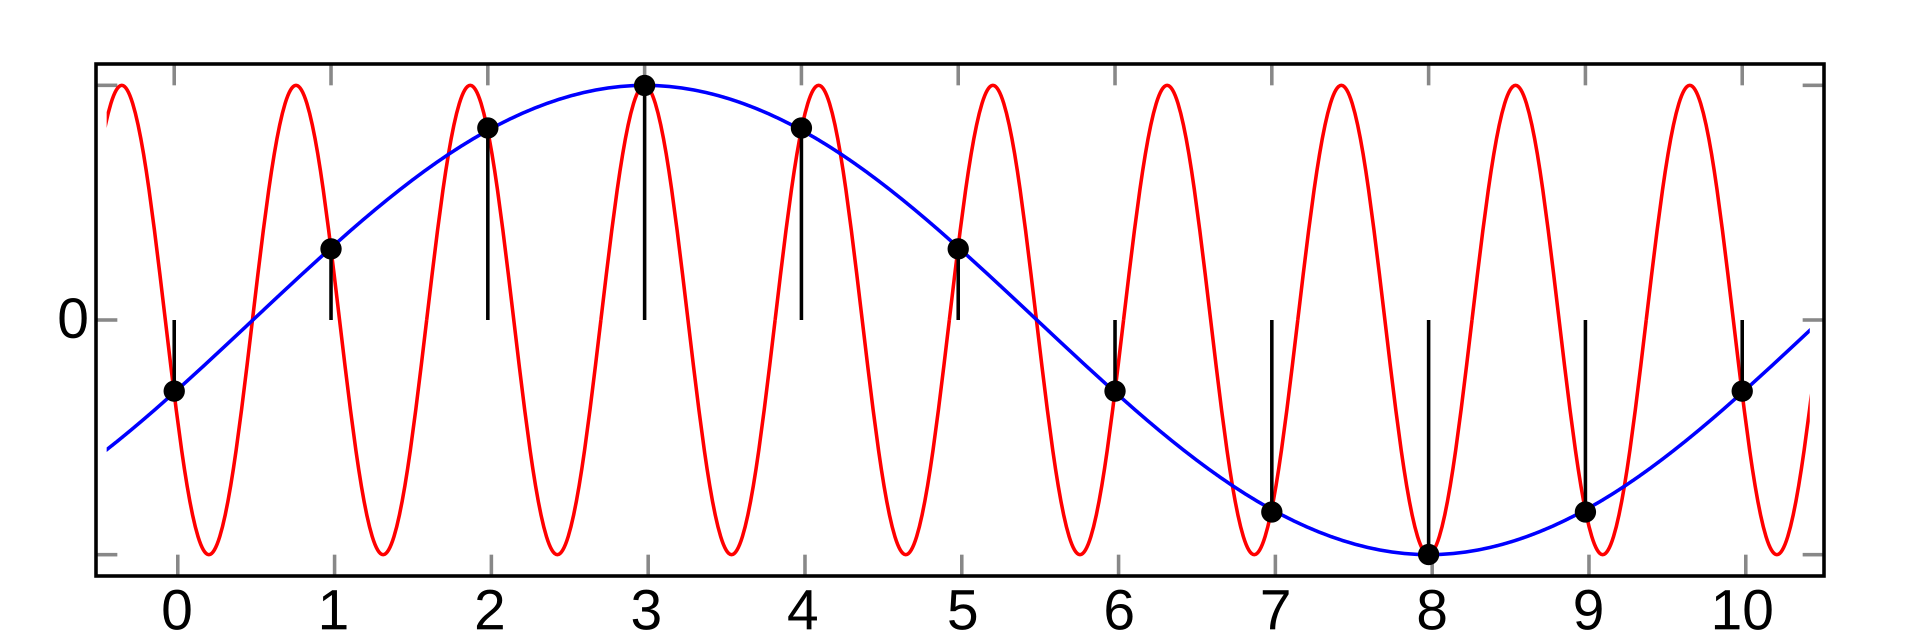
\includegraphics[width=\linewidth]{../figures/d3_aliasing.png}\\
\credit{Moxfyre, CC BY-SA 3.0, via Wikimedia Commons}\\[1mm]
{\scriptsize red: $f=0.9$, blue: $f=0.1$, sampled at $f_s=1$ --- identical samples}
\end{column}
\begin{column}{.48\textwidth}
\footnotesize
\begin{eqbox}
\[ f_{\text{alias}}=\left|f-k\,f_s\right|,\quad k=\operatorname{round}(f/f_s) \]
\end{eqbox}
\begin{itemize}\setlength\itemsep{.4mm}
\item anything above $f_s/2$ folds back into $[0,f_s/2]$
\item \textbf{example:} 4.6\,kHz structural/switching component sampled at 4\,kHz $\Rightarrow$ appears at \hl{600\,Hz} --- inside the loop's range
\item after sampling it cannot be separated: filter \emph{before} the sampler
\item remedies: analogue RC anti-alias filter, oversampling + decimation, sampling synchronous to the PWM centre
\end{itemize}
\begin{notebox}
More in Day 5 (sensing and signal acquisition).
\end{notebox}
\end{column}
\end{columns}
\end{frame}

% --------------------------------------------------------------------
\begin{frame}{Choosing the sample rate}
\begin{columns}[T]
\begin{column}{.52\textwidth}
\centering
\begin{tikzpicture}
\begin{axis}[mkplot,width=7.5cm,height=5.4cm,xmin=0,xmax=30,ymin=0,ymax=2.0,xlabel={$t$ [ms]},ylabel={$\omega/\omega_{\text{ref}}$},
   legend style={at={(0.97,0.97)},anchor=north east}]
\addplot[mkBlue,thick] table[x=t,y=w]{data/fs_20000.dat};\addlegendentry{$f_s=20$\,kHz (14\,\%)}
\addplot[mkOrange,thick] table[x=t,y=w]{data/fs_4000.dat};\addlegendentry{$f_s=4$\,kHz (16\,\%)}
\addplot[mkRed,thick] table[x=t,y=w]{data/fs_1000.dat};\addlegendentry{$f_s=1$\,kHz (95\,\%)}
\draw[mkGray,densely dashed] (axis cs:0,1) -- (axis cs:30,1);
\end{axis}
\end{tikzpicture}
\end{column}
\begin{column}{.46\textwidth}
\footnotesize
Same velocity PI ($f_c=100$\,Hz, $J=\SI{2e-3}{kg\,m^2}$), discrete, 1-sample calculation delay.\\[1mm]
At 1\,kHz: $T_d=1.5$\,ms $\Rightarrow\Delta\varphi=54^\circ$ $\Rightarrow$ near-unstable.
\begin{keybox}[Rules of thumb]
\begin{itemize}\setlength\itemsep{.3mm}
\item $f_s\ge 20$--$40\times$ closed-loop bandwidth for near-continuous behaviour
\item check $360^\circ f_cT_d$ fits the PM budget
\item nested loops: inner loops sample faster
\item sensor and PWM rate must match $f_s$
\end{itemize}
\end{keybox}
\end{column}
\end{columns}
\src{[Franklin, Powell \& Workman, 1998, ch.~11]; simulation for this course.}
\end{frame}

% --------------------------------------------------------------------
\begin{frame}{Session 2.9 summary}
\begin{columns}[T]
\begin{column}{.55\textwidth}
\begin{keybox}[Key take-aways]
\footnotesize
\begin{itemize}\setlength\itemsep{.5mm}
\item Sampling + ZOH + calculation $\approx1.5T$ delay $\Rightarrow$ phase loss $360^\circ f_cT_d$.
\item Stability in $z$: all poles inside the unit circle; $z=e^{sT}$.
\item Tustin for controllers (pre-warp notches), ZOH-equivalent for plants, avoid forward Euler for fast poles.
\item Discrete PID: backward-Euler I, filtered D on measurement, anti-windup, saturation.
\item Filter analogue signals before sampling (aliasing).
\item Choose $f_s$ from the bandwidth \emph{and} the phase budget.
\end{itemize}
\end{keybox}
\end{column}
\begin{column}{.43\textwidth}
\scriptsize
\begin{tabular}{@{}lc@{}}
\toprule
$f_s$ (with $f_c=200$\,Hz) & $\Delta\varphi$ at $T_d=1.5T$\\
\midrule
2\,kHz & $54^\circ$\\
4\,kHz & $27^\circ$\\
8\,kHz & $13.5^\circ$\\
16\,kHz & $6.8^\circ$\\
\bottomrule
\end{tabular}
\vspace{2mm}
\begin{notebox}
Next: how these loops are stacked inside a real servo drive.
\end{notebox}
\end{column}
\end{columns}
\end{frame}

% ####################################################################
\section{3.1 Servo System Architecture}
% ####################################################################

\begin{frame}{Servo system architecture: from mains to load}
\begin{columns}[T]
\begin{column}{.68\textwidth}
\centering
\vspace{-2mm}\begin{tikzpicture}[node distance=4mm]
  \node[blk,minimum height=9mm] (Mains) {mains\\3$\sim$ 400\,V};
  \node[blk,right=of Mains,minimum height=9mm] (PS) {power\\supply};
  \node[blk,right=5mm of PS,minimum width=22mm,minimum height=19mm,fill=mkLight,anchor=west,yshift=-3mm] (Dr) {};
  \node[font=\tiny\bfseries,text=mkBlue,anchor=north] at (Dr.north) {servo drive};
  \node[blkO,font=\tiny,minimum height=4mm,anchor=north] (Ctl) at ($(Dr.north)+(0,-3.6mm)$) {pos./vel./current ctrl};
  \node[blk,font=\tiny,minimum height=4mm,below=1mm of Ctl] (Inv) {DC bus + inverter};
  \node[blk,right=6mm of Dr.east,anchor=west,minimum height=9mm,yshift=3mm] (M) {motor};
  \node[blk,right=of M,minimum height=9mm] (Tr) {transmission\\\tiny gear / screw};
  \node[blk,right=of Tr,minimum height=9mm] (L) {load};
  \node[blkO,below=5mm of M,minimum height=5mm] (Enc) {feedback\\\tiny encoder};
  \node[blk,above=5mm of Dr,minimum height=6mm] (MC) {motion controller\\\tiny PLC / CNC};
  \draw[sig,line width=1pt] (Mains) -- (PS);
  \draw[sig,line width=1pt] (PS) -- (PS -| Dr.west) node[pos=.5,above,font=\tiny]{DC};
  \draw[sig,line width=1pt,mkOrange] (Dr.east |- M) -- (M) node[pos=.4,above,font=\tiny,text=mkNavy]{U V W};
  \draw[line width=1.2pt,mkNavy] (M) -- (Tr);
  \draw[line width=1.2pt,mkNavy] (Tr) -- (L);
  \draw[mkNavy,densely dotted] (M) -- (Enc);
  \draw[sig,mkMid] (Enc) -| ($(Dr.south east)+(-3mm,0)$);
  \draw[sig,mkMid,{Latex[length=1.5mm]}-{Latex[length=1.5mm]}] (MC) -- (Dr) node[pos=.5,right,font=\tiny]{fieldbus (EtherCAT \dots)};
\end{tikzpicture}
\vspace{2mm}

\footnotesize
\begin{itemize}\setlength\itemsep{.3mm}
\item \term{drive} = power stage + control loops + protection; \term{feedback} closes every loop
\item the motion controller sends set-points (position/velocity/torque) every 0.25--4\,ms
\end{itemize}
\end{column}
\begin{column}{.30\textwidth}
\centering
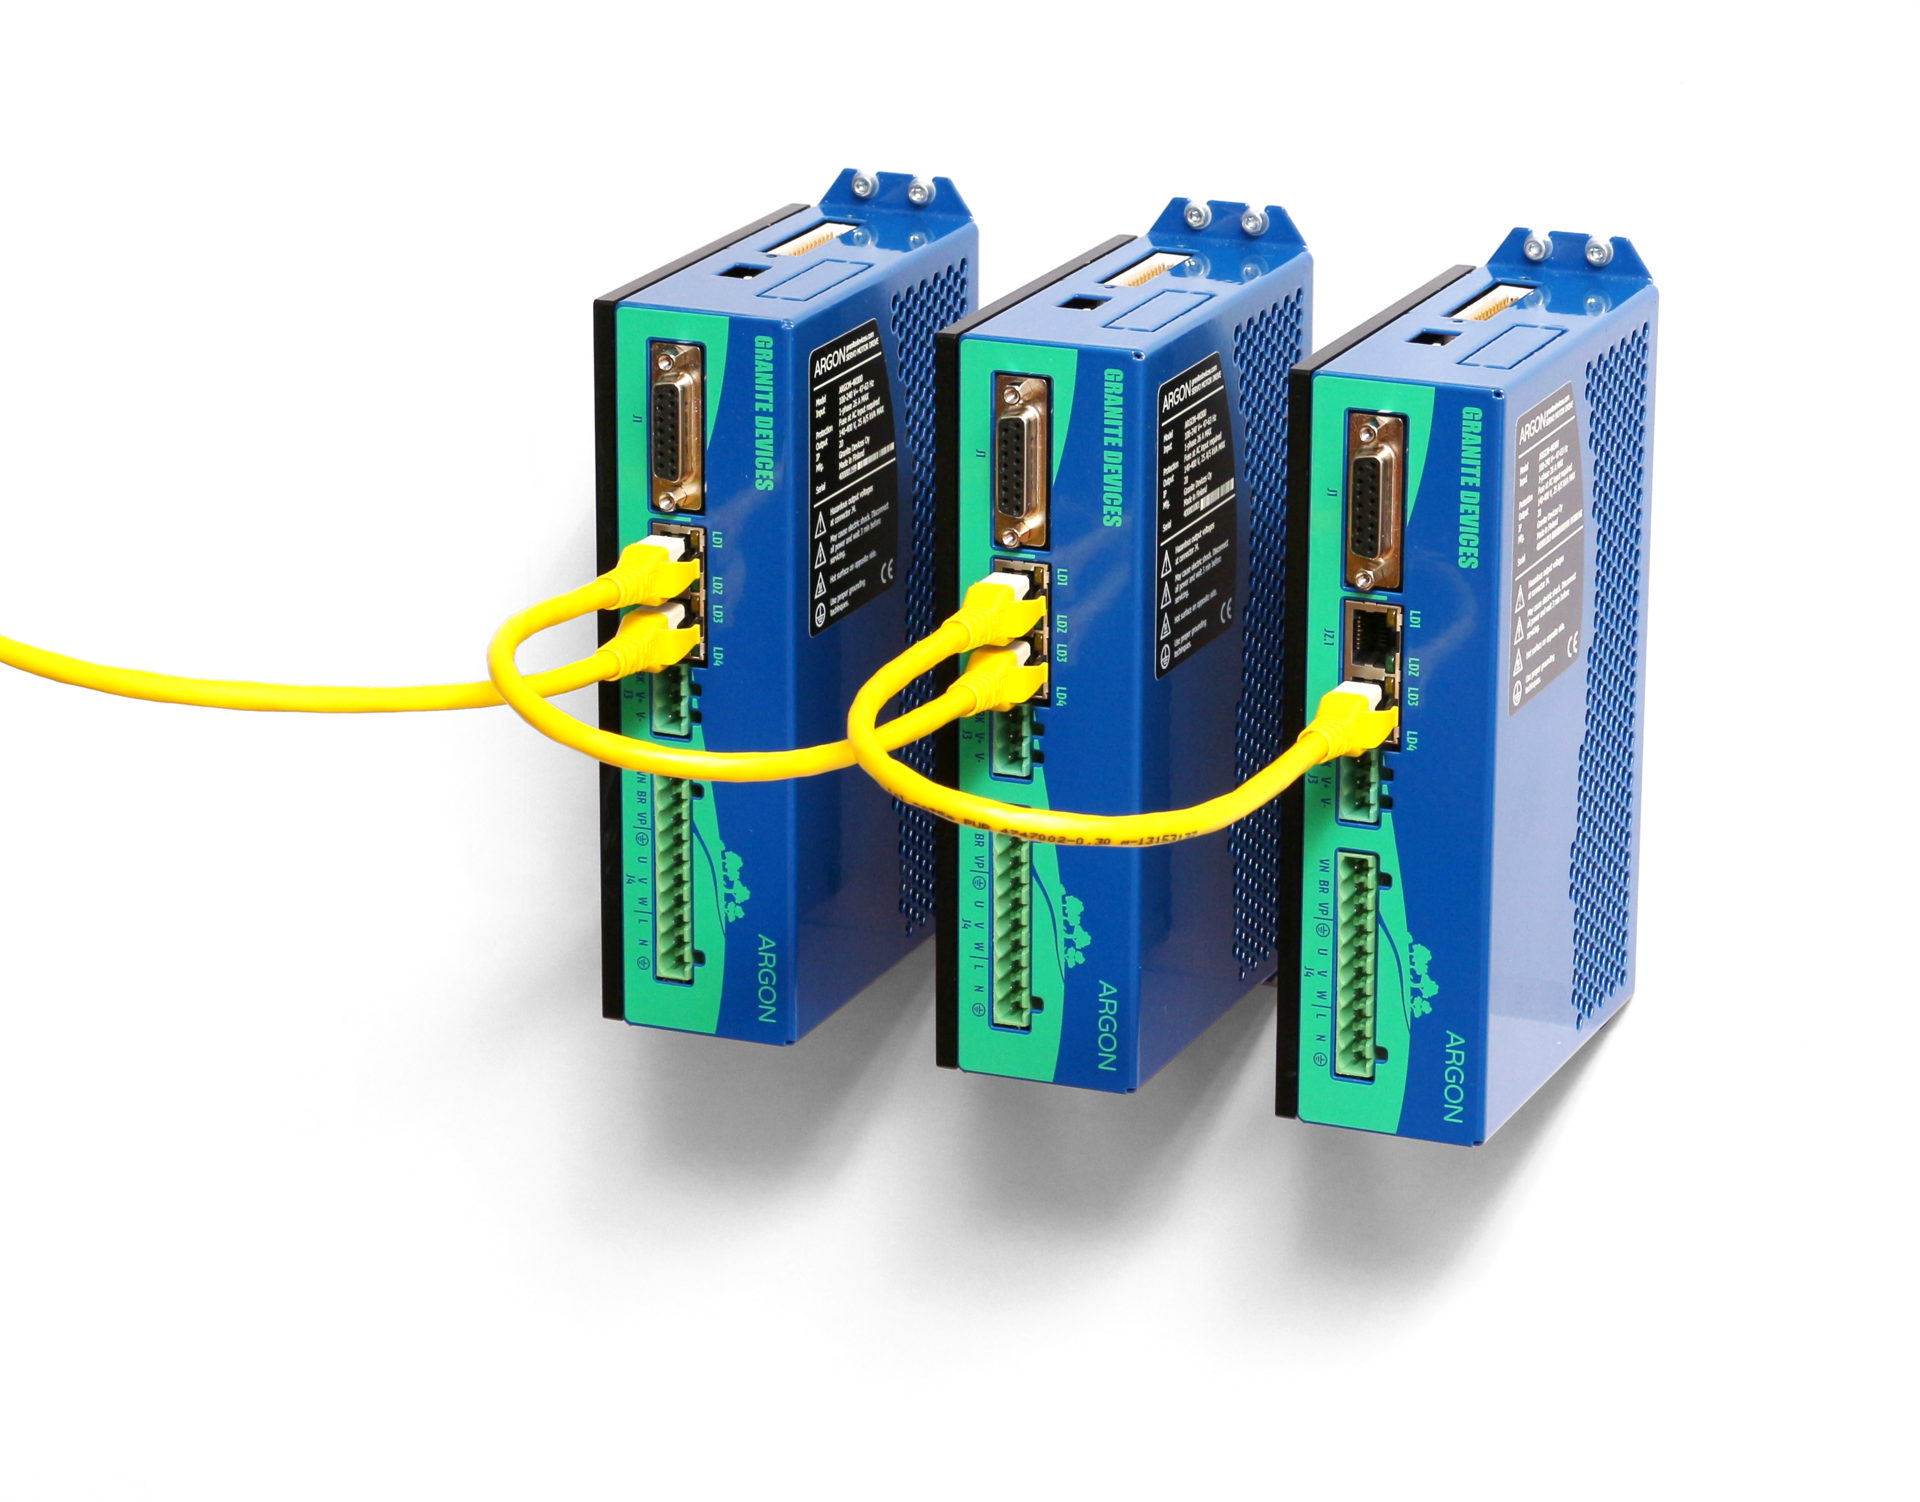
\includegraphics[width=.85\linewidth]{../figures/d3_servo_drives.png}\\
\credit{Tero Kontkanen, CC BY-SA 3.0, via Wikimedia Commons}\\[1mm]
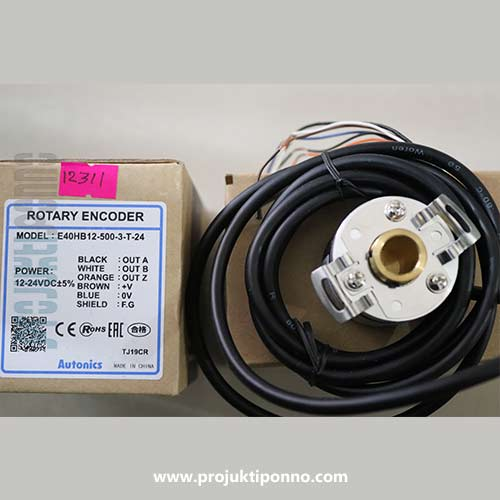
\includegraphics[width=.38\linewidth]{../figures/d3_encoder.jpg}\\
\credit{Projuktiponno, CC BY-SA 4.0, via Wikimedia Commons}\\
{\tiny compact servo drives on a daisy-chained fieldbus; incremental encoder}
\end{column}
\end{columns}
\end{frame}

% --------------------------------------------------------------------
\begin{frame}{Torque, velocity and position control modes}
\scriptsize
\begin{tabularx}{\textwidth}{@{}l X X l X@{}}
\toprule
\textbf{Mode} & \textbf{Command from controller} & \textbf{Loops closed in the drive} & \textbf{Typ.\ BW} & \textbf{Applications}\\
\midrule
Torque (current) & $T^*$ or $i_q^*$ & current loop only & 1--3\,kHz & winders/tension, press-fit force, master--slave torque sharing\\
Velocity & $\omega^*$ & velocity + current & 100--500\,Hz & spindles, conveyors, CNC with position loop in the controller\\
Position & $\theta^*$ (or profile) & position + velocity + current & 20--100\,Hz & point-to-point, robots, synchronised axes\\
\bottomrule
\end{tabularx}
\vspace{2mm}
\begin{columns}[T]
\begin{column}{.52\textwidth}
\footnotesize
\textbf{Where is each loop closed?}
\begin{itemize}\setlength\itemsep{.3mm}
\item cyclic synchronous modes (CiA\,402 / IEC\,61800-7): \term{CSP}, \term{CSV}, \term{CST} --- set-points every cycle
\item profile modes (PP, PV): the drive generates the trajectory itself
\item the faster the inner loop, the closer it must sit to the power stage
\end{itemize}
\end{column}
\begin{column}{.46\textwidth}
\begin{keybox}[Selection rule]
\footnotesize
Close a loop where its \textbf{sensor} and its \textbf{update rate} are; send the controller only what it can update fast enough.
\end{keybox}
\end{column}
\end{columns}
\end{frame}

% --------------------------------------------------------------------
\begin{frame}{Cascade control structure of a servo drive}
\centering
\begin{tikzpicture}[node distance=4.5mm]
  \node[sumn] (Sp) {\sumsym};
  \node[blk,right=of Sp] (Cp) {$K_{pp}$\\[-.5mm]\tiny position P};
  \node[sumn,right=6mm of Cp] (Sv) {\sumsym};
  \node[blk,right=of Sv] (Cv) {PI\\[-.5mm]\tiny velocity};
  \node[sumn,right=6mm of Cv] (Si) {\sumsym};
  \node[blk,right=of Si] (Ci) {PI\\[-.5mm]\tiny current};
  \node[blkO,right=of Ci] (Inv) {PWM\\inverter};
  \node[blk,right=of Inv] (Mot) {$\frac{1}{Ls+R}$\\[-.5mm]\tiny winding};
  \node[blk,right=of Mot] (Kt) {$k_t$};
  \node[blk,right=of Kt] (Mech) {$\frac{1}{Js}$};
  \node[blk,right=of Mech] (Int) {$\frac1s$};
  \draw[sig] ($(Sp.west)+(-5mm,0)$) node[left,font=\scriptsize]{$\theta^*$} -- (Sp);
  \draw[sig] (Sp) -- (Cp); \draw[sig] (Cp) -- (Sv); \draw[sig] (Sv) -- node[above,font=\tiny]{} (Cv);
  \draw[sig] (Cv) -- (Si); \draw[sig] (Si) -- (Ci); \draw[sig] (Ci) -- (Inv);
  \draw[sig] (Inv) -- node[above,font=\tiny]{$v$} (Mot); \draw[sig] (Mot) -- node[above,font=\tiny]{$i$} (Kt);
  \draw[sig] (Kt) -- node[above,font=\tiny]{$T_m$} (Mech); \draw[sig] (Mech) -- node[above,font=\tiny]{$\omega$} (Int);
  \draw[sig] (Int.east) -- ++(4mm,0) node[right,font=\scriptsize]{$\theta$};
  \draw[sig] ($(Int.east)+(2mm,0)$) -- ++(0,-14mm) -| node[pos=.97,left,font=\tiny]{$-$} (Sp);
  \draw[sig] ($(Mech.east)!.5!(Int.west)$) -- ++(0,-9mm) -| node[pos=.95,left,font=\tiny]{$-$} (Sv);
  \draw[sig] ($(Mot.east)!.5!(Kt.west)$) -- ++(0,-4.5mm) -| node[pos=.9,left,font=\tiny]{$-$} (Si);
  % feedforward
  \draw[sig,mkOrange,densely dashed] ($(Sp.west)+(-3mm,0)$) -- ++(0,9mm) -| node[pos=.25,above,font=\tiny,text=mkOrange]{velocity feed-forward $\dot\theta^*$} (Sv.north);
  \draw[sig,mkOrange,densely dashed] ($(Sp.west)+(-3mm,9mm)$) -- ++(0,6mm) -| node[pos=.2,above,font=\tiny,text=mkOrange]{torque/acceleration feed-forward $\hat J\ddot\theta^*$} (Si.north);
  \node[font=\tiny,text=mkGray,below=13mm of Cv] {velocity feedback $\omega$ (encoder, differentiated/observed)};
\end{tikzpicture}
\vspace{1mm}
\begin{columns}[T]
\begin{column}{.5\textwidth}
\footnotesize
\begin{itemize}\setlength\itemsep{.3mm}
\item each inner loop makes the outer plant simple: current loop $\to$ ``torque source'', velocity loop $\to$ ``integrator''
\item bandwidth separation \hl{3--10$\times$} between loops
\end{itemize}
\end{column}
\begin{column}{.48\textwidth}
\footnotesize
\begin{itemize}\setlength\itemsep{.3mm}
\item feed-forwards give tracking without high feedback gains
\item tuned inside-out: current $\to$ velocity $\to$ position
\end{itemize}
\end{column}
\end{columns}
\src{[Ellis, 2012, ch.~17]; [Leonhard, 2001].}
\end{frame}

% --------------------------------------------------------------------
\begin{frame}{Session 3.1 summary: the bandwidth hierarchy}
\begin{columns}[T]
\begin{column}{.52\textwidth}
\centering
\begin{tikzpicture}
\begin{axis}[mkplot,xmode=log,width=7.6cm,height=5.2cm,xmin=1,xmax=30000,ymin=-40,ymax=6,xlabel={$f$ [Hz]},ylabel={closed-loop $|T|$ [dB]},
   legend style={at={(0.02,0.03)},anchor=south west}]
\addplot[mkMid,thick] table[x=f,y=pc]{data/bw.dat};\addlegendentry{position ($\approx40$\,Hz)}
\addplot[mkOrange,thick] table[x=f,y=vc]{data/bw.dat};\addlegendentry{velocity ($\approx250$\,Hz)}
\addplot[mkBlue,thick] table[x=f,y=ic]{data/bw.dat};\addlegendentry{current ($\approx2$\,kHz)}
\draw[mkGray,densely dashed] (axis cs:1,-3) -- (axis cs:30000,-3);
\end{axis}
\end{tikzpicture}
\end{column}
\begin{column}{.46\textwidth}
\begin{keybox}[Key take-aways]
\footnotesize
\begin{itemize}\setlength\itemsep{.4mm}
\item Servo = supply + drive + motor + transmission + load + feedback + motion controller.
\item Three modes: torque, velocity, position --- defined by which loops the drive closes.
\item Cascade: current $\gg$ velocity $\gg$ position bandwidth (factor 3--10 each).
\item Feed-forward for tracking, feedback for disturbances.
\end{itemize}
\end{keybox}
\end{column}
\end{columns}
\end{frame}

% ####################################################################
\section{3.2 Power Electronics I: Rectifier, DC Bus and Inverter}
% ####################################################################

\begin{frame}{Power stage of a servo drive: overview}
\begin{columns}[T]
\begin{column}{.77\textwidth}
\centering
\resizebox{\linewidth}{!}{%
\begin{circuitikz}[scale=1,transform shape,line width=.6pt]
\ctikzset{bipoles/length=.85cm,diodes/scale=.8}
% rails
\draw (1,3) -- (2.9,3); \draw (1,0) -- (11.4,0);
% rectifier legs
\foreach \x in {1,1.8,2.6}{
  \draw (\x,1.85) to[D*] (\x,3);
  \draw (\x,0) to[D*] (\x,1.15);
  \draw (\x,1.15) -- (\x,1.85);
}
\draw (1,3) -- (2.6,3);
\draw (-0.3,1.7) node[ocirc,label={[font=\scriptsize]left:L1}]{} -- (1,1.7) node[circ]{};
\draw (-0.3,1.5) node[ocirc,label={[font=\scriptsize]left:L2}]{} -- (1.8,1.5) node[circ]{};
\draw (-0.3,1.3) node[ocirc,label={[font=\scriptsize]left:L3}]{} -- (2.6,1.3) node[circ]{};
\node[font=\scriptsize,text=mkBlue] at (1.8,3.55) {diode rectifier};
% precharge
\draw (2.6,3) -- (3.0,3) to[R,l=\scriptsize$R_{pc}$] (4.4,3) -- (4.8,3);
\draw (3.0,3) -- (3.0,3.7) to[nos,l=\scriptsize bypass] (4.4,3.7) -- (4.4,3);
% DC link
\draw (4.8,3) -- (5.4,3) to[eC,l_=\scriptsize$C_{dc}$] (5.4,0);
\draw (5.0,2.6) node[font=\scriptsize,text=mkOrange]{$+$};
\draw[mkOrange,-{Latex[length=1.6mm]}] (4.75,0.4) -- (4.75,2.4) node[midway,left,font=\scriptsize,text=mkOrange]{$V_{dc}$};
% brake chopper
\draw (5.4,3) -- (6.6,3) to[R,l=\scriptsize$R_b$] (6.6,1.7);
\draw (6.6,1.7) node[nigbt,anchor=C,scale=.8](Tb){};
\draw (Tb.E) -- (6.6,0);
\node[font=\scriptsize,text=mkBlue] at (6.6,3.55) {brake chopper};
% inverter legs
\draw (6.6,3) -- (10.6,3);
\foreach \x/\n in {8.0/a,9.3/b,10.6/c}{
  \draw (\x,3) node[nigbt,anchor=C,scale=.8](T\n u){};
  \draw (T\n u.E) -- (\x,1.35);
  \draw (\x,1.35) node[nigbt,anchor=C,scale=.8](T\n l){};
  \draw (T\n l.E) -- (\x,0);
  \draw (T\n u.C) -- ++(0.45,0) to[D*,diodes/scale=.6] ($(T\n u.E)+(0.45,0)$) -- (T\n u.E);
  \draw (T\n l.C) -- ++(0.45,0) to[D*,diodes/scale=.6] ($(T\n l.E)+(0.45,0)$) -- (T\n l.E);
}
\node[font=\scriptsize,text=mkBlue] at (9.3,3.55) {three-phase inverter};
% outputs
\coordinate (ua) at (8.0,1.75); \coordinate (ub) at (9.3,1.6); \coordinate (uc) at (10.6,1.45);
\draw (ua) node[circ]{} -- (11.9,1.75); \draw (ub) node[circ]{} -- (11.9,1.6); \draw (uc) node[circ]{} -- (11.9,1.45);
\draw[fill=mkPale,draw=mkBlue,thick] (12.45,1.6) circle (0.5) node[font=\small]{M};
\node[font=\tiny] at (11.75,1.95) {U V W};
\end{circuitikz}}
\end{column}
\begin{column}{.21\textwidth}
\centering
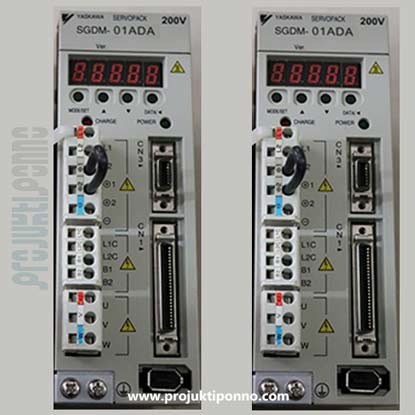
\includegraphics[width=\linewidth]{../figures/d3_servo_drive_motor.jpg}\\
\credit{Projuktiponno, CC BY-SA 4.0, via Wikimedia Commons}\\[1mm]
{\tiny Terminals: L1/L2(/L3) mains, L1C/L2C control supply, B1/B2 brake resistor, $\oplus/\ominus$ DC bus, U/V/W motor}
\end{column}
\end{columns}
\vspace{1mm}
\footnotesize
\textbf{AC $\to$ DC $\to$ AC:} uncontrolled rectifier charges the DC link; pre-charge resistor limits inrush; the brake chopper dumps regenerated energy; the two-level inverter synthesises variable-voltage, variable-frequency three-phase voltages by PWM.
\end{frame}

% --------------------------------------------------------------------
\begin{frame}{Rectifier and DC link}
\begin{columns}[T]
\begin{column}{.5\textwidth}
\centering
\begin{tikzpicture}
\begin{axis}[mkplot,width=7.3cm,height=4.4cm,xmin=0,xmax=40,ymin=-600,ymax=650,xlabel={$t$ [ms]},ylabel={[V]},
  ytick={-565,0,540,565},yticklabels={$-566$,0,540,566},legend style={at={(0.98,0.03)},anchor=south east}]
\foreach \c in {ab,bc,ca,ba,cb,ac} {\addplot[mkSky,thin,forget plot] table[x=t,y=\c]{data/rect.dat};}
\addplot[mkOrange,very thick] table[x=t,y=dc]{data/rect.dat};\addlegendentry{$v_{dc}$ (no capacitor)}
\draw[mkBlue,densely dashed] (axis cs:0,540) -- (axis cs:40,540);
\end{axis}
\end{tikzpicture}
\scriptsize
6-pulse output = envelope of the six line-to-line voltages; ripple at $6f=\SI{300}{Hz}$.
\end{column}
\begin{column}{.48\textwidth}
\footnotesize
\begin{eqbox}
\[ V_{dc,\text{avg}}=\frac{3\sqrt2}{\pi}V_{LL}=1.35\,V_{LL},\qquad \hat V=\sqrt2\,V_{LL} \]
\end{eqbox}
400\,V mains: 540\,V average, 566\,V peak (light load, capacitor charges to peak).
\begin{itemize}\setlength\itemsep{.2mm}
\item $C_{dc}$: ripple current, energy buffer, low-inductance commutation loop
\item pre-charge resistor + bypass relay: limit inrush into an empty $C_{dc}$
\item diode front end is \hl{not regenerative}
\end{itemize}
\vspace{-1mm}
\begin{center}
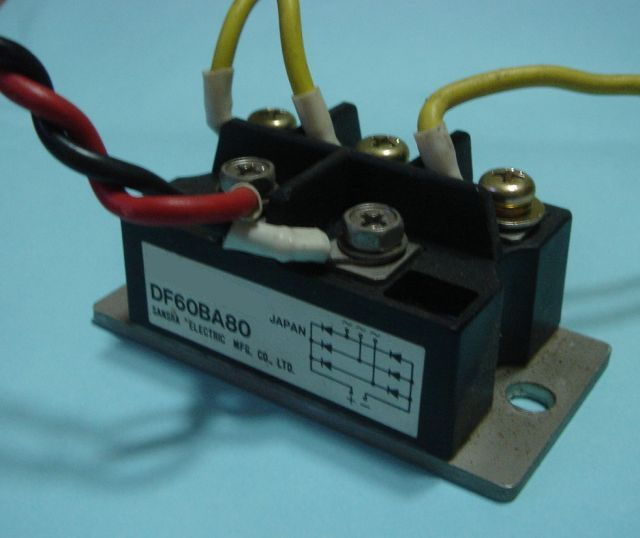
\includegraphics[height=1.55cm]{../figures/d3_diode_module.jpg}\hspace{1mm}
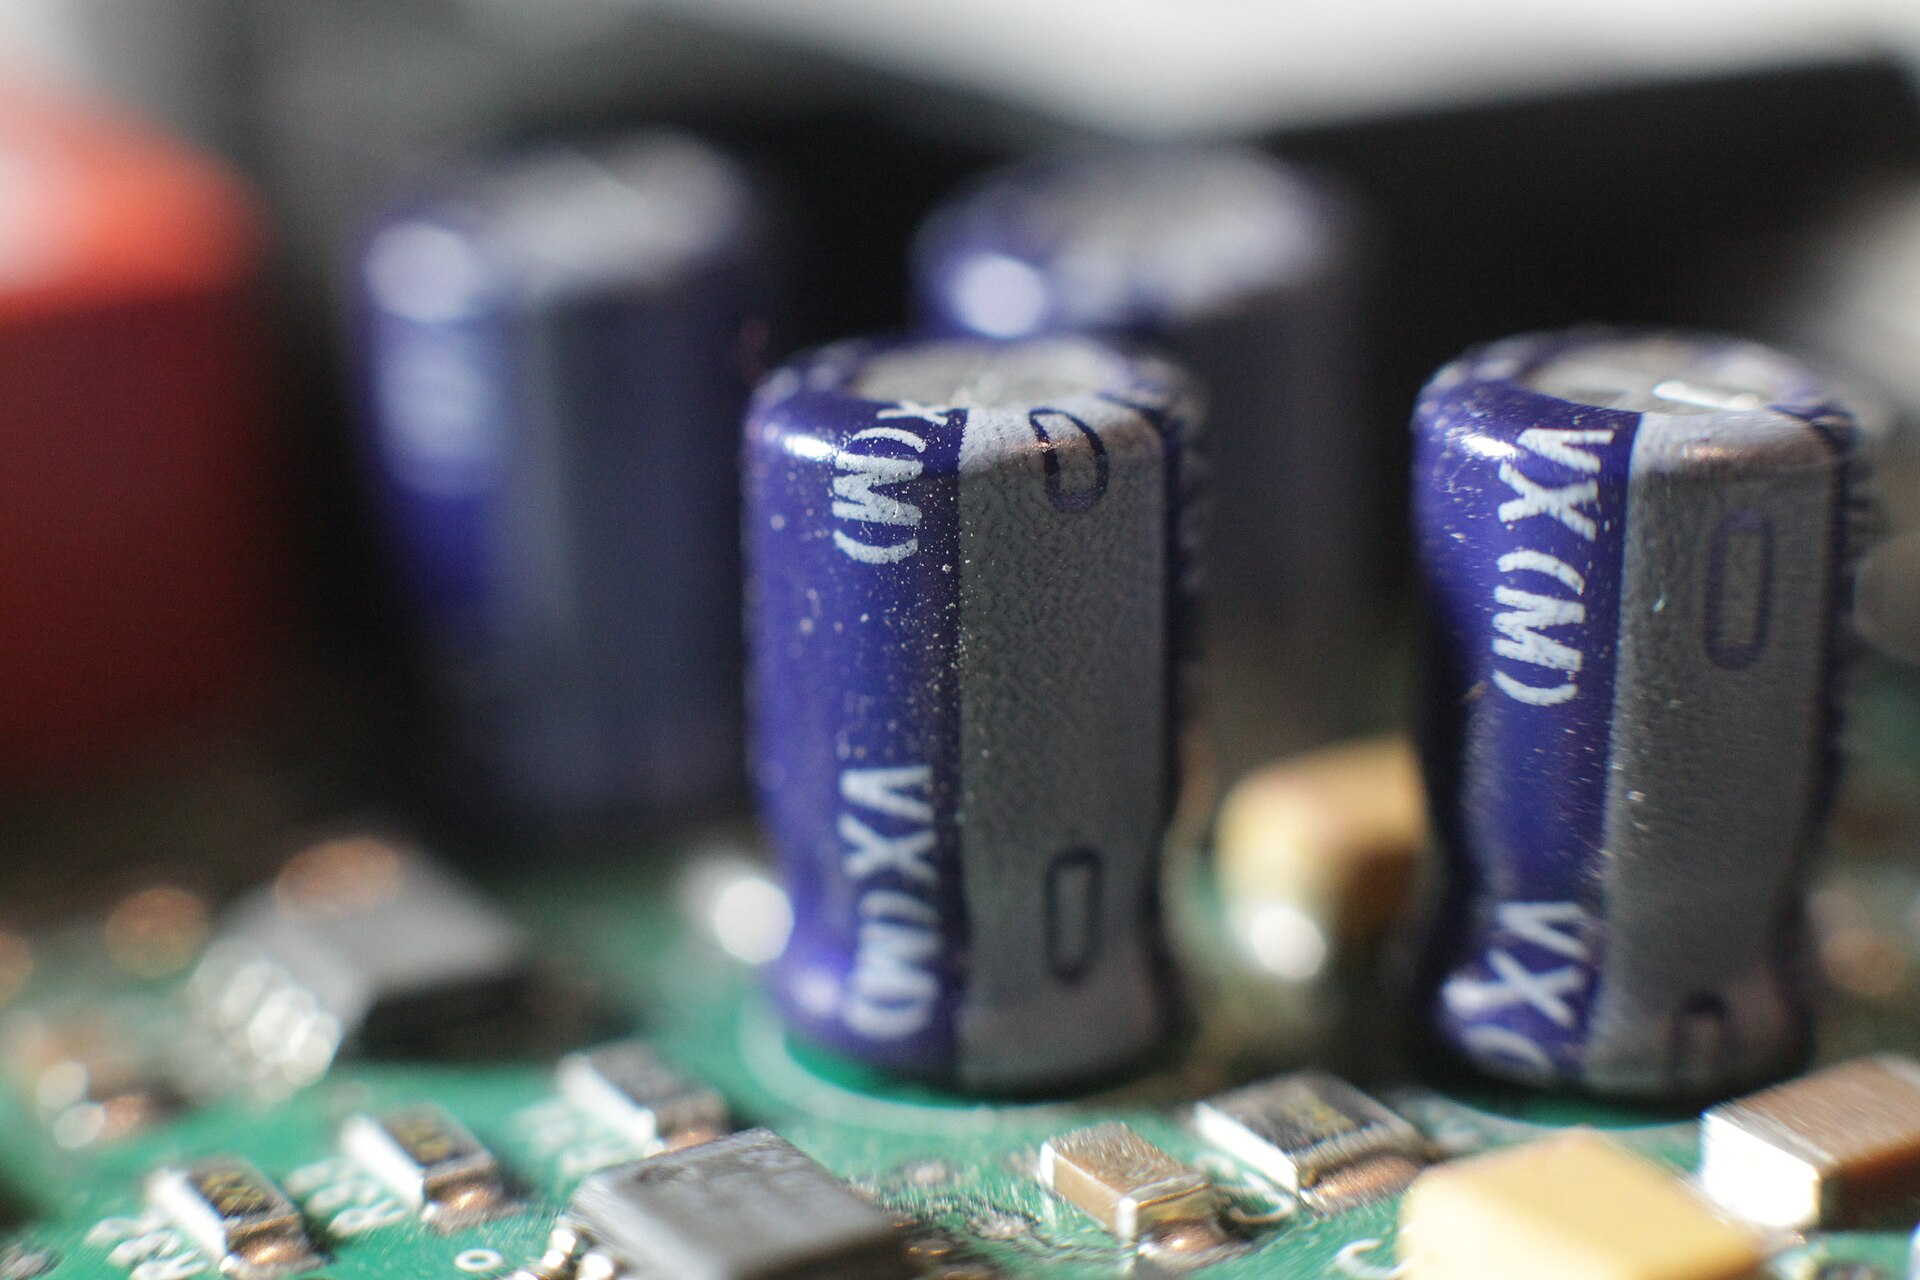
\includegraphics[height=1.55cm]{../figures/d3_dclink_caps.jpg}\\
\credit{left: Hiro36, CC BY-SA 3.0; right: Giovanna 27, CC BY 4.0; via Wikimedia Commons}
\end{center}
\end{column}
\end{columns}
\end{frame}

% --------------------------------------------------------------------
\begin{frame}{Regeneration and the brake chopper}
\begin{columns}[T]
\begin{column}{.47\textwidth}
\scriptsize
\textbf{Worked example.} $J=\SI{0.05}{kg\,m^2}$ decelerated linearly from 3000\,rpm ($\SI{314}{rad/s}$) to 0 in 0.5\,s:
\begin{itemize}\setlength\itemsep{.2mm}
\item kinetic energy $E=\tfrac12J\omega^2=\SI{2467}{J}$
\item torque $J\alpha=\SI{31.4}{N\,m}$, peak power $P=T\omega=\SI{9.87}{kW}$
\item $C_{dc}=\SI{1}{mF}$ from 565 to 780\,V absorbs only $\tfrac12C(780^2-565^2)=\SI{145}{J}$ (6\,\%)
\item resistor must take peak power at $V_{on}$: $R_b\le V_{on}^2/P=\SI{61.6}{\ohm}$ $\Rightarrow$ choose \hl{56\,$\Omega$}
\end{itemize}
\vspace{-1mm}
\begin{center}
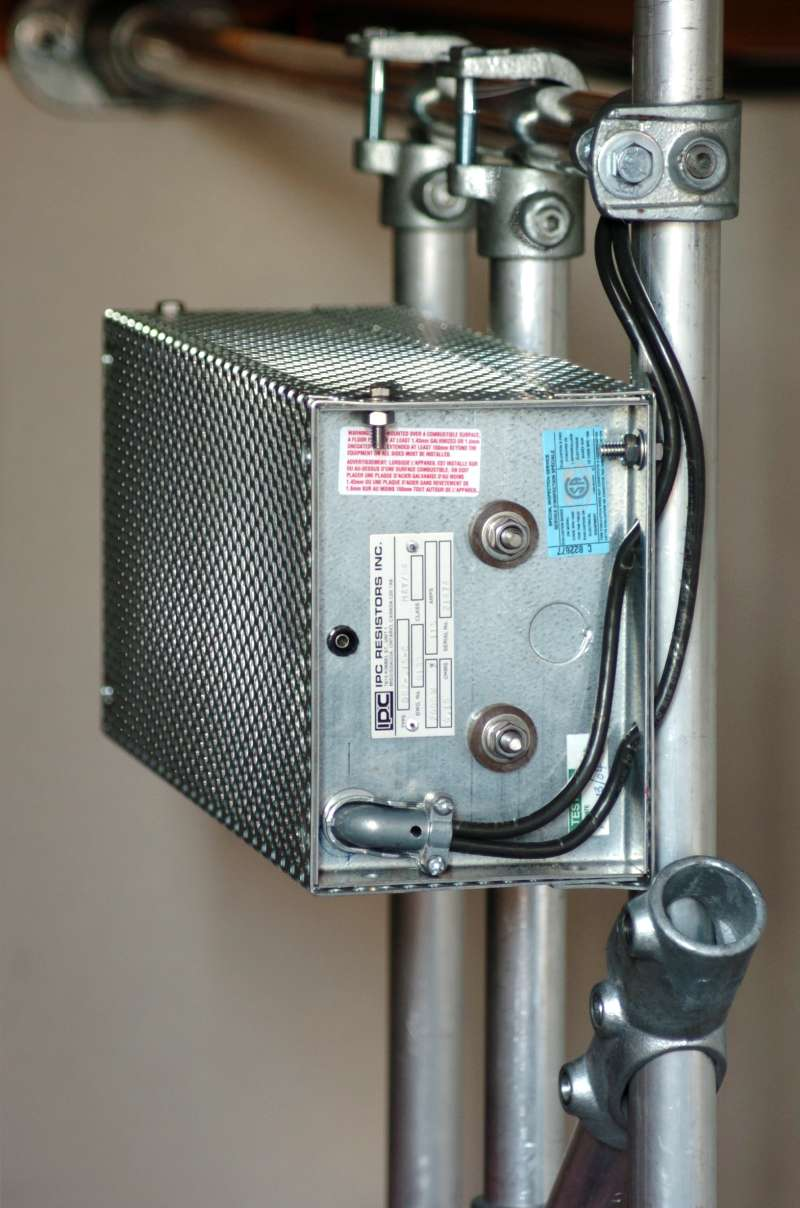
\includegraphics[height=2.0cm]{../figures/d3_brake_resistor.jpg}\\
\credit{Glogger, CC BY-SA 3.0, via Wikimedia Commons}
\end{center}
\end{column}
\begin{column}{.51\textwidth}
\centering
\begin{tikzpicture}
\begin{groupplot}[group style={group size=1 by 2,vertical sep=2mm,xticklabels at=edge bottom},mkplot,width=7.3cm,xmin=0,xmax=700]
\nextgroupplot[height=3.9cm,ylabel={$V_{dc}$ [V]},ymin=540,ymax=820,ytick={565,760,780}]
\addplot[mkOrange,thin] table[x=t,y=v]{data/vdc_brake.dat};
\draw[mkRed,densely dashed] (axis cs:0,780) -- (axis cs:700,780);
\nextgroupplot[height=2.5cm,ylabel={$P_{\text{regen}}$ [kW]},xlabel={$t$ [ms]},ymin=0,ymax=11]
\addplot[mkBlue,thick] table[x=t,y=p]{data/vdc_brake.dat};
\end{groupplot}
\end{tikzpicture}
\scriptsize
Hysteresis chopper: on at 780\,V, off at 760\,V. Alternatives: common DC bus between axes, active (regenerative) front end.
\end{column}
\end{columns}
\end{frame}

% --------------------------------------------------------------------
\begin{frame}{Three-phase two-level inverter}
\begin{columns}[T]
\begin{column}{.5\textwidth}
\centering
\begin{circuitikz}[scale=.78,transform shape,line width=.6pt]
\draw (0,3.2) -- (4.6,3.2); \draw (0,0) -- (4.6,0);
\draw (0,3.2) to[eC] (0,1.6) to[eC] (0,0);
\draw (0,1.6) node[circ]{} node[left,font=\scriptsize]{N\,} ;
\node[font=\scriptsize,anchor=east] at (-0.3,3.2) {$+\frac{V_{dc}}{2}$};
\node[font=\scriptsize,anchor=east] at (-0.3,0) {$-\frac{V_{dc}}{2}$};
\foreach \x/\n/\p in {1.4/a/1,2.8/b/3,4.2/c/5}{
  \draw (\x,3.2) node[nigbt,anchor=C](U\n){};
  \draw (U\n.E) -- (\x,1.4);
  \draw (\x,1.4) node[nigbt,anchor=C](L\n){};
  \draw (L\n.E) -- (\x,0);
  \node[font=\tiny,anchor=east] at ($(U\n.G)+(-0.05,0)$) {$S_{\n}^{+}$};
  \node[font=\tiny,anchor=east] at ($(L\n.G)+(-0.05,0)$) {$S_{\n}^{-}$};
}
\draw (1.4,1.85) node[circ]{} -- (5.3,1.85) node[right,font=\scriptsize]{$a$};
\draw (2.8,1.65) node[circ]{} -- (5.3,1.65) node[right,font=\scriptsize]{$b$};
\draw (4.2,1.45) node[circ]{} -- (5.3,1.45) node[right,font=\scriptsize]{$c$};
\end{circuitikz}

{\tiny\color{mkGray}antiparallel (freewheeling) diodes omitted for clarity --- see photo}
\end{column}
\begin{column}{.48\textwidth}
\footnotesize
\begin{itemize}\setlength\itemsep{.3mm}
\item each leg ties its phase to $+V_{dc}/2$ or $-V_{dc}/2$: \term{two-level}
\item $S^+$ and $S^-$ of a leg switch \hl{complementarily} --- never both on
\item $2^3=8$ switching states: 6 active, 2 zero vectors
\item average leg voltage set by duty: $\bar v_{aN}=(2d_a-1)V_{dc}/2$
\item freewheeling diodes carry current during dead time and regeneration
\end{itemize}
\begin{center}
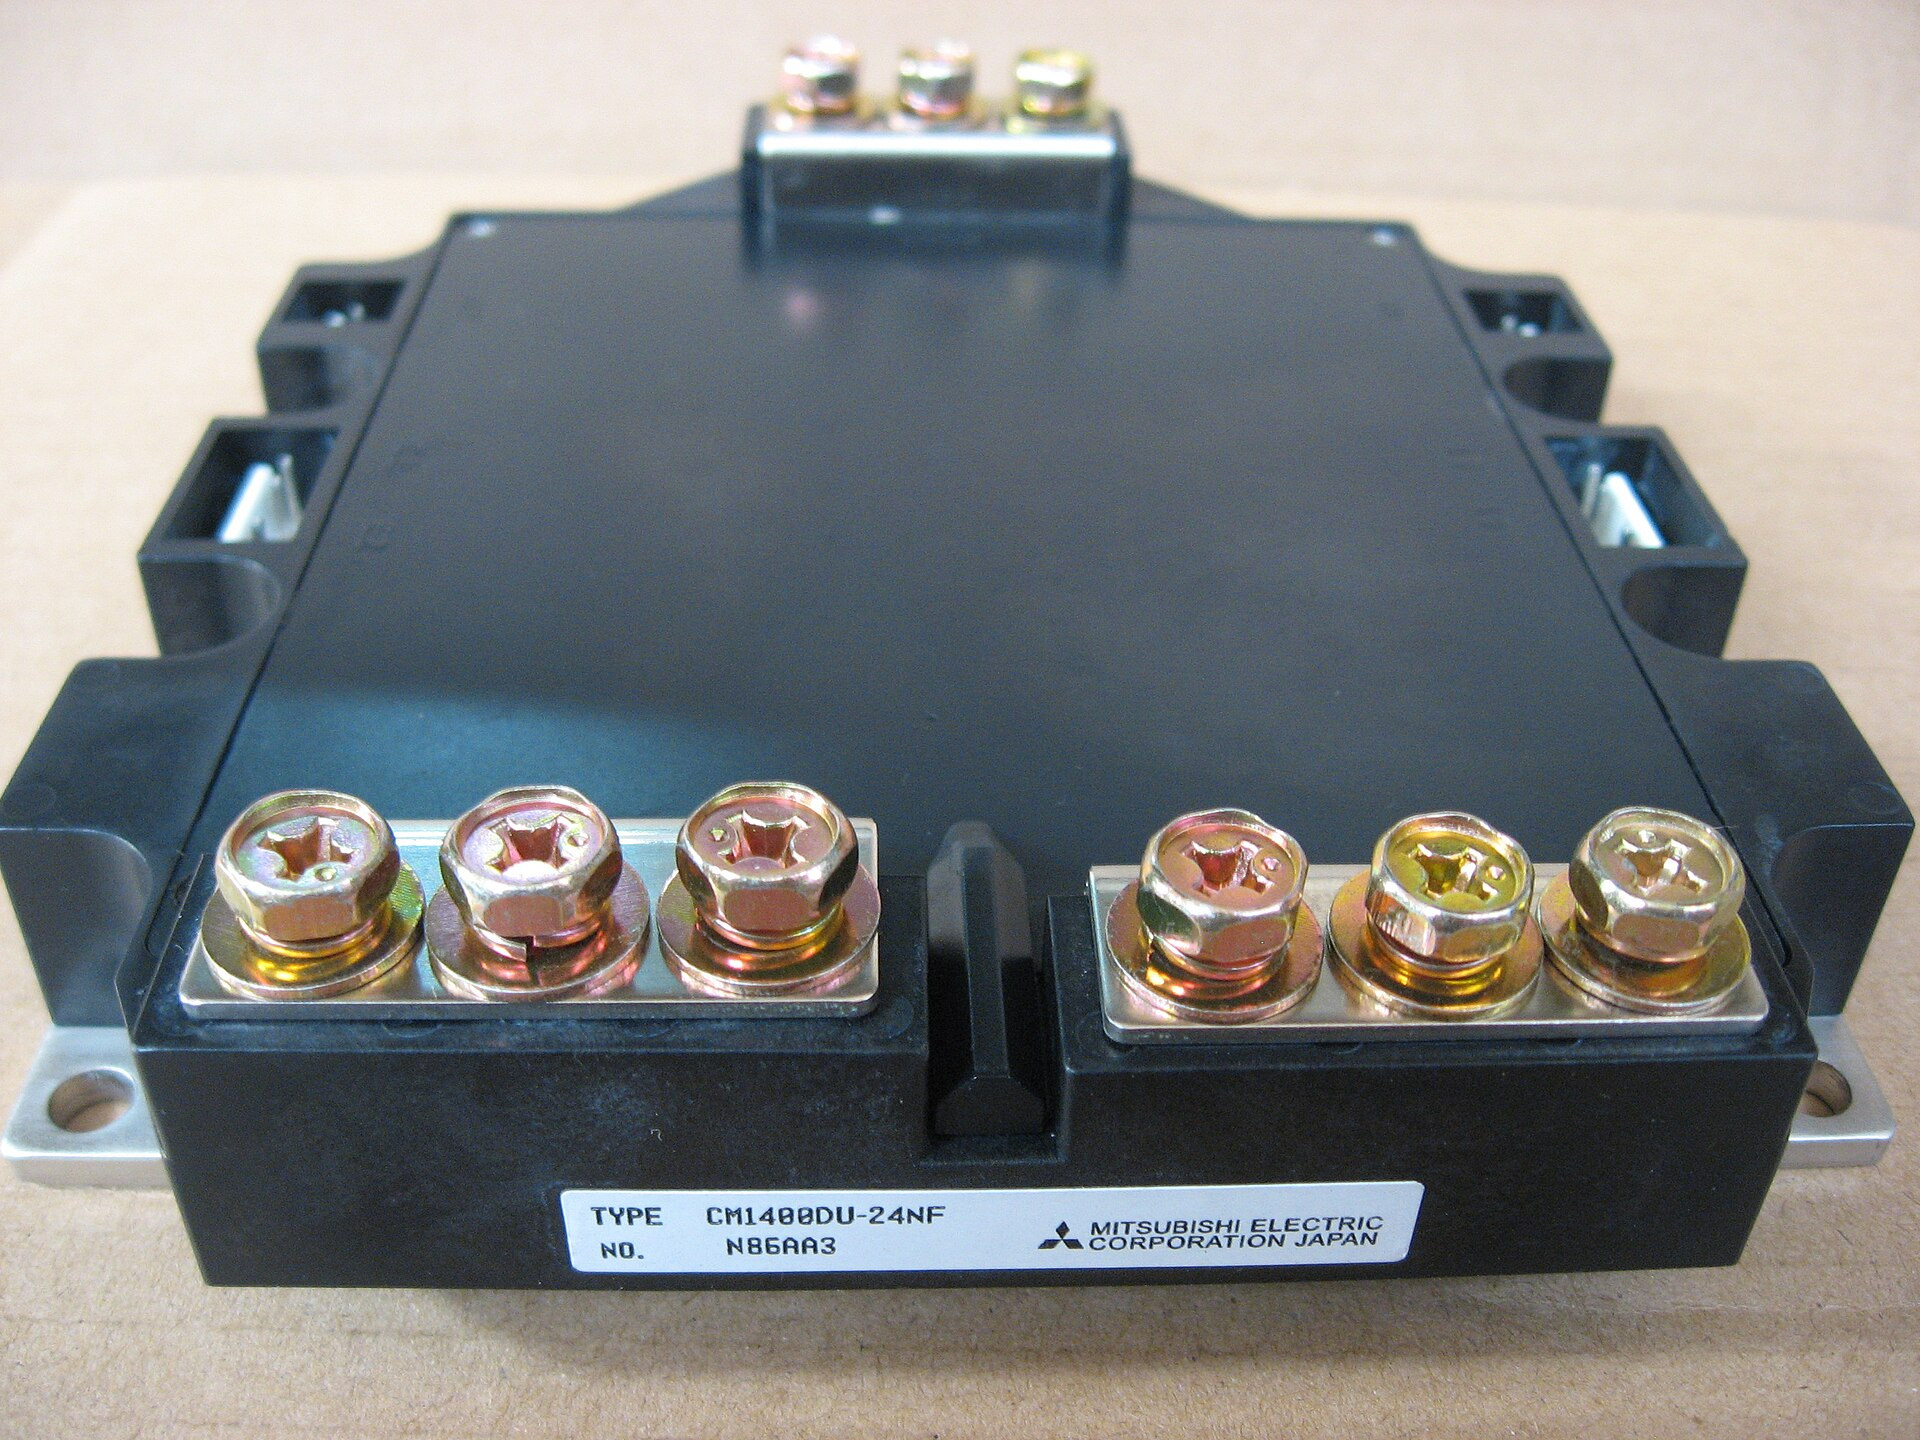
\includegraphics[height=1.9cm]{../figures/d3_igbt_module.jpg}\\
\credit{Sthdhk, CC BY-SA 4.0, via Wikimedia Commons}\\
{\tiny dual (half-bridge) IGBT module}
\end{center}
\end{column}
\end{columns}
\end{frame}

% --------------------------------------------------------------------
\begin{frame}{Power switches: IGBT, MOSFET and wide band-gap}
\begin{columns}[T]
\begin{column}{.64\textwidth}
\scriptsize
\begin{tabularx}{\linewidth}{@{}l X X X@{}}
\toprule
 & \textbf{Si IGBT} & \textbf{Si MOSFET} & \textbf{SiC MOSFET}\\
\midrule
voltage class & 600--1700\,V & $\le$ 250\,V (low-voltage drives) & 650--1700\,V\\
conduction & $V_{CE(sat)}\approx1.5$--2\,V & $R_{DS(on)}$: m$\Omega$ & $R_{DS(on)}$, low\\
switching & tail current, slower & very fast & very fast\\
typ.\ $f_{sw}$ & 4--16\,kHz & 20--100\,kHz & 16--100\,kHz\\
servo use & 400\,V industrial drives & 24--72\,V axes, robots, AGVs & compact/high-$f_s$ drives\\
\bottomrule
\end{tabularx}
\vspace{2mm}
\footnotesize
\begin{itemize}\setlength\itemsep{.3mm}
\item higher $f_{sw}$ $\Rightarrow$ less current ripple, faster current loop, smaller filters
\item but high $dv/dt$ stresses motor insulation and causes bearing currents and EMI
\end{itemize}
\end{column}
\begin{column}{.34\textwidth}
\centering
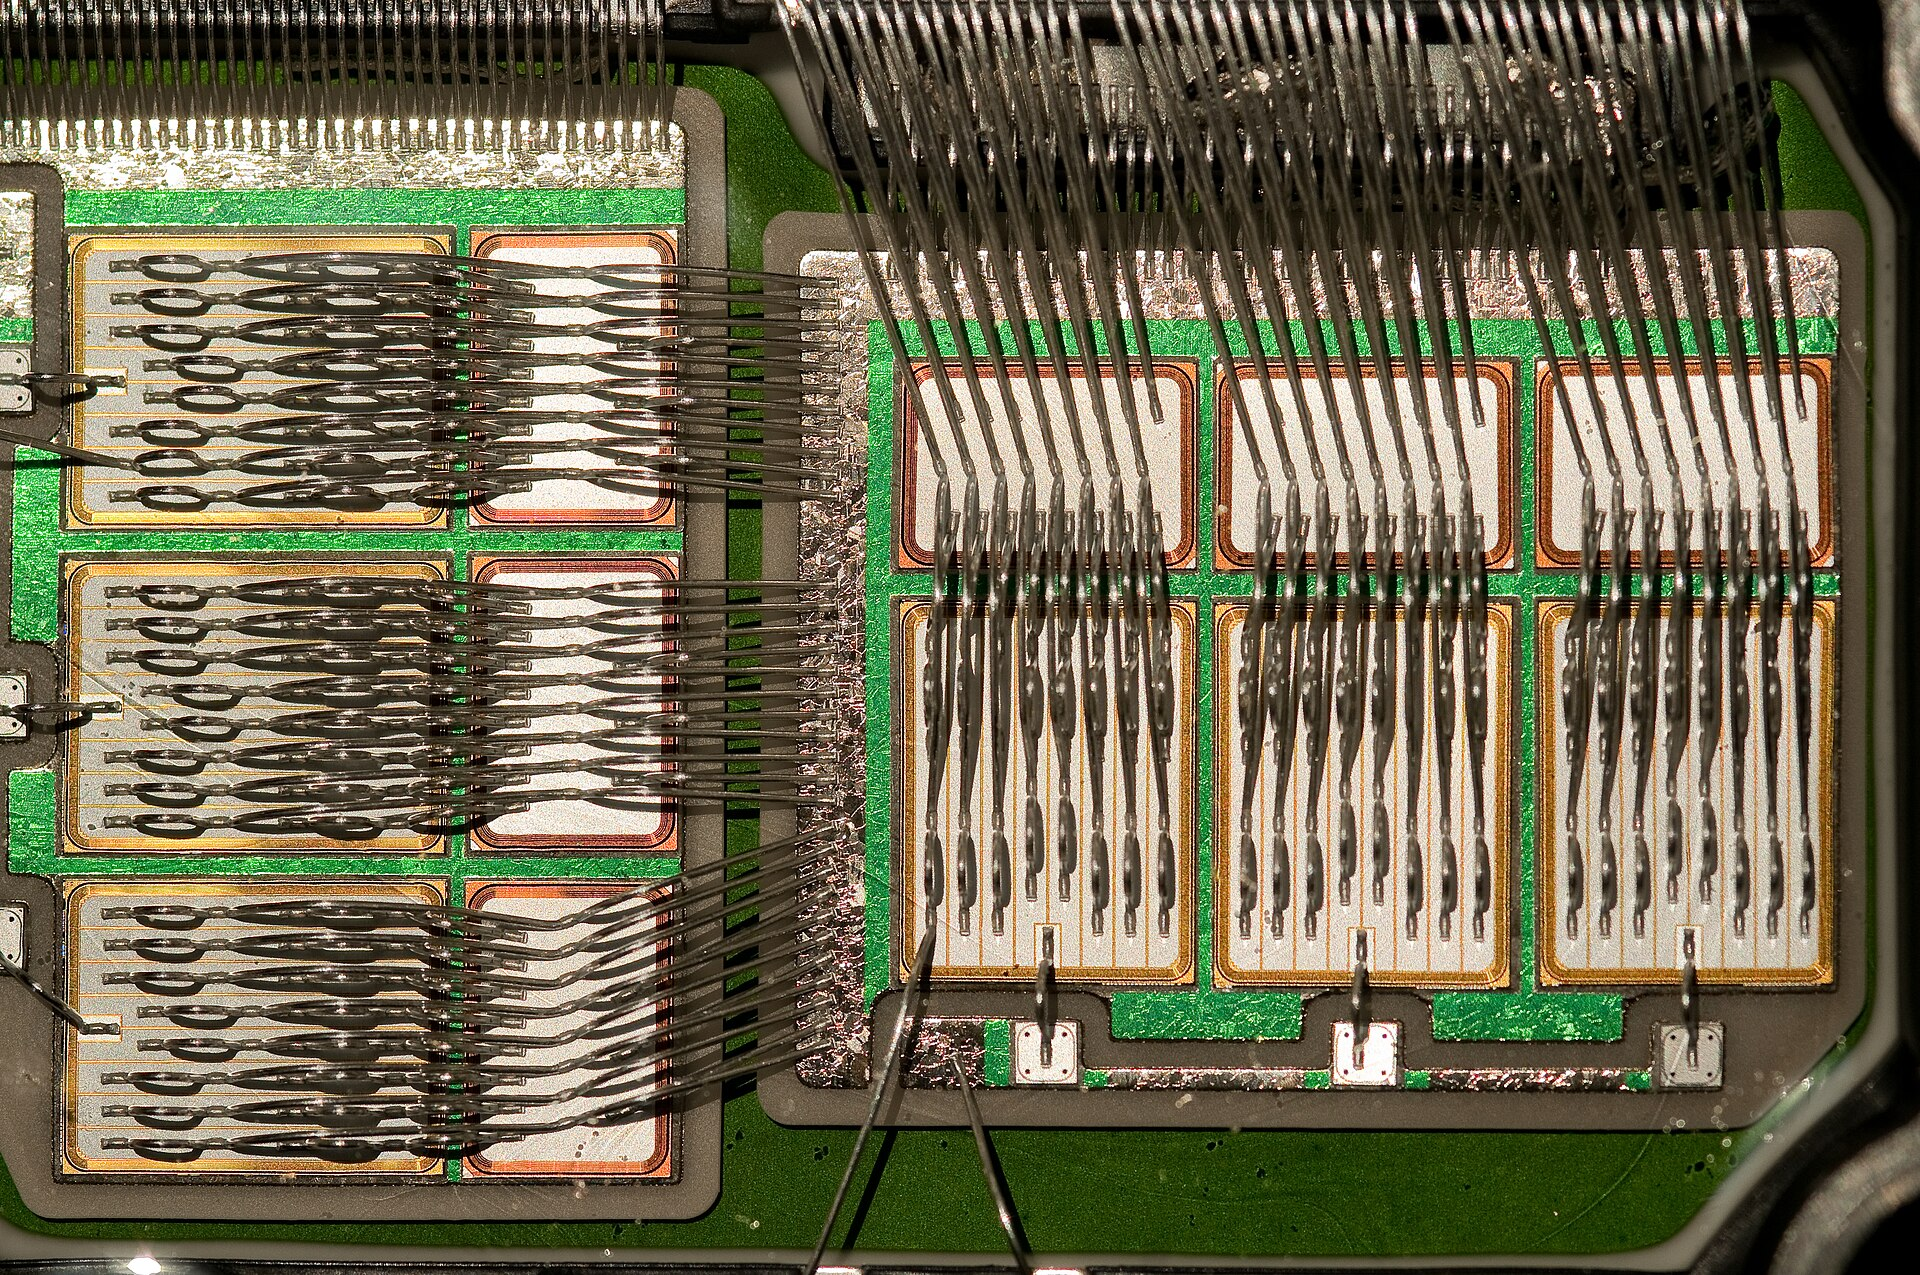
\includegraphics[width=\linewidth]{../figures/d3_igbt_module_open.jpg}\\
\credit{Pslawinski, CC BY-SA 3.0, via Wikimedia Commons}\\
{\tiny opened IGBT module: paralleled IGBT dies and freewheeling diodes with bond wires}
\end{column}
\end{columns}
\src{[Mohan, Undeland \& Robbins, 2003, ch.~8 \& 22]; [Krishnan, 2001].}
\end{frame}

% --------------------------------------------------------------------
\begin{frame}{Gate drivers and dead time (preview)}
\begin{columns}[T]
\begin{column}{.43\textwidth}
\footnotesize
\textbf{Gate driver functions}
\begin{itemize}\setlength\itemsep{.3mm}
\item level shift / \term{galvanic isolation} for the high-side switch (bootstrap or isolated supply)
\item peak gate current of several A; typical IGBT drive $+15$\,V / $-8$\,V
\item \term{desaturation} (short-circuit) detection, soft turn-off within $\approx\SI{10}{\micro s}$
\item Miller clamp, under-voltage lock-out
\end{itemize}
\textbf{Dead time} $t_d$: both switches off after each transition to prevent \hl{shoot-through}.
\end{column}
\begin{column}{.55\textwidth}
\centering
\begin{tikzpicture}[x=1cm,y=1cm]
  \tikzset{wave/.style={mkBlue,thick}}
  \node[font=\tiny,anchor=east] at (0,2.9) {ideal};
  \draw[wave] (0,2.7) -- (1,2.7) -- (1,3.1) -- (4,3.1) -- (4,2.7) -- (5.6,2.7);
  \node[font=\tiny,anchor=east] at (0,2.1) {$S^+$};
  \draw[wave,mkOrange] (0,1.9) -- (1.4,1.9) -- (1.4,2.3) -- (4,2.3) -- (4,1.9) -- (5.6,1.9);
  \node[font=\tiny,anchor=east] at (0,1.3) {$S^-$};
  \draw[wave,mkOrange] (0,1.5) -- (1,1.5) -- (1,1.1) -- (4.4,1.1) -- (4.4,1.5) -- (5.6,1.5);
  \fill[mkRed,opacity=.2] (1,0.2) rectangle (1.4,3.2);
  \fill[mkRed,opacity=.2] (4,0.2) rectangle (4.4,3.2);
  \node[font=\tiny,text=mkRed] at (1.2,3.4) {$t_d$};
  \node[font=\tiny,text=mkRed] at (4.2,3.4) {$t_d$};
  \node[font=\tiny,anchor=east] at (0,0.5) {$v_{aN}$, $i>0$};
  \draw[wave,mkMid] (0,0.3) -- (1.4,0.3) -- (1.4,0.7) -- (4.4,0.7) -- (4.4,0.3) -- (5.6,0.3);
  \draw[mkGray,densely dashed] (1,0.2) -- (1,0.8); \draw[mkGray,densely dashed] (4,0.2) -- (4,0.8);
\end{tikzpicture}\par
\vspace{1mm}
\scriptsize
During $t_d$ the diode conducts, so $v_{aN}$ depends on the \emph{current sign}: for $i>0$ the pulse is shortened by $t_d$.
\begin{eqbox}
\[ \Delta\bar v\approx\frac{t_d}{T_{sw}}\,V_{dc}\,\operatorname{sign}(i) \]
\end{eqbox}
\textbf{Example:} $t_d=\SI{2}{\micro s}$, $f_{sw}=10$\,kHz, $V_{dc}=560$\,V $\Rightarrow\Delta\bar v=$ \hl{11.2\,V} --- distortion at low speed; compensation on Day 4.
\end{column}
\end{columns}
\src{[Balogh, TI SLUA618]; [Mohan, Undeland \& Robbins, 2003].}
\end{frame}

% --------------------------------------------------------------------
\begin{frame}{Session 3.2 (part 1) summary}
\begin{columns}[T]
\begin{column}{.55\textwidth}
\begin{keybox}[Key take-aways]
\footnotesize
\begin{itemize}\setlength\itemsep{.5mm}
\item Drive power path: rectifier $\to$ pre-charge $\to$ DC link $\to$ brake chopper $\to$ inverter $\to$ motor.
\item $V_{dc}\approx1.35V_{LL}$ (540\,V at 400\,V mains).
\item Braking energy mostly exceeds what $C_{dc}$ can store: size $R_b$ from $V_{on}^2/P_{\text{peak}}$.
\item Two-level inverter: 8 states, complementary switching per leg.
\item Gate driver: isolation, protection; dead time prevents shoot-through but costs volts.
\end{itemize}
\end{keybox}
\end{column}
\begin{column}{.43\textwidth}
\scriptsize
\begin{tabular}{@{}ll@{}}
\toprule
\textbf{Quantity} & \textbf{Value (400\,V drive)}\\
\midrule
$V_{dc}$ nominal & 540--565\,V\\
chopper on & $\approx$780\,V\\
over-voltage trip & $\approx$800--850\,V\\
IGBT class & 1200\,V\\
$f_{sw}$ & 4--16\,kHz\\
dead time & 0.5--3\,\textmu s\\
\bottomrule
\end{tabular}

{\tiny\color{mkGray}typical orders of magnitude; check the specific drive datasheet}
\end{column}
\end{columns}
\end{frame}

% ====================================================================  closing
\section*{Wrap-up}
\begin{frame}{Day 3 summary}
\begin{columns}[T]
\begin{column}{.5\textwidth}
\footnotesize
\begin{defbox}[Control]
\begin{itemize}\setlength\itemsep{.3mm}
\item in-loop filters cost phase; notches tame resonances; lead adds PM, lag adds stiffness
\item state feedback + observer: pole placement, separation, integral state, LQR
\item robust: $|WT|<1$; adaptive: MRAC with MIT or Lyapunov laws; scheduling and DOB in practice
\item digital: $T_d\approx1.5T$, $z=e^{sT}$, Tustin + pre-warp, anti-windup
\end{itemize}
\end{defbox}
\end{column}
\begin{column}{.48\textwidth}
\footnotesize
\begin{defbox}[Servo hardware]
\begin{itemize}\setlength\itemsep{.3mm}
\item servo = drive + motor + transmission + feedback + motion controller
\item torque / velocity / position modes, cascaded loops with feed-forward
\item rectifier, DC link, brake chopper, two-level inverter, gate drivers, dead time
\end{itemize}
\end{defbox}
\begin{keybox}[One sentence]
\footnotesize
The achievable servo bandwidth is set by phase: filters, delay and resonances spend it, compensators and fast sampling buy it back.
\end{keybox}
\end{column}
\end{columns}
\end{frame}

\begin{frame}{Preview of Day 4}
\begin{columns}[T]
\begin{column}{.55\textwidth}
\footnotesize
\textbf{Day 4 --- Servo drives in depth}
\begin{itemize}\setlength\itemsep{.5mm}
\item PWM techniques: sinusoidal PWM, space-vector modulation, over-modulation
\item dead-time effects and compensation (continuing today's preview)
\item field-oriented control: Clarke/Park transforms, $i_d$/$i_q$ current loops, decoupling
\item current, velocity and position loop tuning in practice
\item feed-forward, resonance handling and auto-tuning in commercial drives
\end{itemize}
\end{column}
\begin{column}{.43\textwidth}
\begin{notebox}
\textbf{Bring with you:} the delay-budget formula $360^\circ f_cT_d$, the notch-filter parameters and the cascade structure --- Day 4 tunes exactly these loops on a PMSM drive.
\end{notebox}
\end{column}
\end{columns}
\end{frame}

\begin{frame}{Figure credits}
\scriptsize
All other diagrams and plots: own drawings, computed for this course (TikZ / pgfplots / circuitikz).\\[1mm]
\begin{tabularx}{\textwidth}{@{}l X l@{}}
\toprule
\textbf{File} & \textbf{Source (Wikimedia Commons)} & \textbf{Author, licence}\\
\midrule
d3\_aliasing.png & File:AliasingSines.svg & Moxfyre, CC BY-SA 3.0\\
d3\_servo\_drives.png & File:Servo motor drive.png & Tero Kontkanen, CC BY-SA 3.0\\
d3\_encoder.jpg & File:Rotary Encoder.jpg & Projuktiponno, CC BY-SA 4.0\\
d3\_servo\_drive\_motor.jpg & File:Yeskawa Servo Drive \& Motor.jpg & Projuktiponno, CC BY-SA 4.0\\
d3\_diode\_module.jpg & File:Diode-module.jpg & Hiro36, CC BY-SA 3.0\\
d3\_dclink\_caps.jpg & File:Electrolytic capacitors mounted on a PCB.jpg & Giovanna 27, CC BY 4.0\\
d3\_brake\_resistor.jpg & File:Turbrake.jpg & Glogger at English Wikipedia, CC BY-SA 3.0\\
d3\_igbt\_module.jpg & File:MITSUBISHI IGBT module.jpg & Sthdhk, CC BY-SA 4.0\\
d3\_igbt\_module\_open.jpg & File:CM600DU-24NFH.jpg & Pslawinski, CC BY-SA 3.0\\
\bottomrule
\end{tabularx}
\end{frame}

\begin{frame}{References}
\fontsize{7}{8.4}\selectfont
\begin{columns}[T]
\begin{column}{.5\textwidth}
\begin{itemize}\setlength\itemsep{.2mm}
\item K.~Ogata, \emph{Modern Control Engineering}, 5th ed., Prentice Hall, 2010.
\item G.~F.~Franklin, J.~D.~Powell, A.~Emami-Naeini, \emph{Feedback Control of Dynamic Systems}, 8th ed., Pearson, 2019.
\item G.~F.~Franklin, J.~D.~Powell, M.~Workman, \emph{Digital Control of Dynamic Systems}, 3rd ed., Addison-Wesley, 1998.
\item K.~J.~{\AA}str\"om, R.~M.~Murray, \emph{Feedback Systems}, 2nd ed., Princeton Univ.\ Press, 2021.
\item K.~J.~{\AA}str\"om, T.~H\"agglund, \emph{Advanced PID Control}, ISA, 2006.
\item K.~J.~{\AA}str\"om, B.~Wittenmark, \emph{Adaptive Control}, 2nd ed., Addison-Wesley, 1995.
\item J.~J.~E.~Slotine, W.~Li, \emph{Applied Nonlinear Control}, Prentice Hall, 1991.
\item P.~A.~Ioannou, J.~Sun, \emph{Robust Adaptive Control}, Prentice Hall, 1996.
\item K.~Zhou, J.~C.~Doyle, K.~Glover, \emph{Robust and Optimal Control}, Prentice Hall, 1996.
\item S.~Skogestad, I.~Postlethwaite, \emph{Multivariable Feedback Control}, 2nd ed., Wiley, 2005.
\item B.~D.~O.~Anderson, J.~B.~Moore, \emph{Optimal Control: Linear Quadratic Methods}, Prentice Hall, 1990.
\end{itemize}
\end{column}
\begin{column}{.5\textwidth}
\begin{itemize}\setlength\itemsep{.2mm}
\item J.~C.~Doyle, ``Guaranteed margins for LQG regulators,'' \emph{IEEE Trans.\ Autom.\ Control}, 23(4), 1978.
\item D.~G.~Luenberger, ``Observing the state of a linear system,'' \emph{IEEE Trans.\ Mil.\ Electron.}, 8(2), 1964.
\item K.~Ohnishi, M.~Shibata, T.~Murakami, ``Motion control for advanced mechatronics,'' \emph{IEEE/ASME Trans.\ Mechatronics}, 1(1), 1996.
\item G.~Ellis, \emph{Control System Design Guide}, 4th ed., Butterworth-Heinemann, 2012.
\item A.~V.~Oppenheim, R.~W.~Schafer, \emph{Discrete-Time Signal Processing}, 3rd ed., Pearson, 2010.
\item N.~Mohan, T.~M.~Undeland, W.~P.~Robbins, \emph{Power Electronics: Converters, Applications and Design}, 3rd ed., Wiley, 2003.
\item R.~Krishnan, \emph{Electric Motor Drives: Modeling, Analysis, and Control}, Prentice Hall, 2001.
\item W.~Leonhard, \emph{Control of Electrical Drives}, 3rd ed., Springer, 2001.
\item L.~Balogh, \emph{Fundamentals of MOSFET and IGBT Gate Driver Circuits}, Texas Instruments, SLUA618.
\item IEC 61800-5-1 (drive safety), IEC 61800-7 (drive profiles, incl.\ CiA\,402).
\end{itemize}
\end{column}
\end{columns}
\end{frame}

\end{document}
